\documentclass[12pt,a4paper]{article}
% Enhanced package selection (copy your setup)
\usepackage[utf8]{inputenc}
\usepackage[T1]{fontenc}
\usepackage{geometry}
\usepackage{graphicx}
\usepackage{fancyhdr}
\usepackage{float}
\usepackage{hyperref}
\usepackage{circuitikz}
\usepackage{caption}
\usepackage{subcaption}
\usepackage{siunitx}
\usepackage{amsmath}
\usepackage{tikz}
\usepackage{booktabs}
\geometry{margin=1in}
\hypersetup{colorlinks=true, linkcolor=orange, urlcolor=orange, citecolor=orange, pdfborder={0 0 0}}

% Custom commands as per your setup
\newcommand{\vecb}[1]{\mathbf{#1}}
\newcommand{\brak}[1]{\ensuremath{\left(#1\right)}}
\newcommand{\cbrak}[1]{\ensuremath{\left\{#1\right\}}}
\newcommand{\abs}[1]{\left\vert#1\right\vert}
\newcommand{\norm}[1]{\left\lVert#1\right\rVert}
\providecommand{\sbrak}[1]{\ensuremath{{}\left[#1\right]}}
\providecommand{\lsbrak}[1]{\ensuremath{{}\left[#1\right.}}
\providecommand{\rsbrak}[1]{\ensuremath{{}\left.#1\right]}}
\providecommand{\brak}[1]{\ensuremath{\left(#1\right)}}
\providecommand{\lbrak}[1]{\ensuremath{\left(#1\right.}}
\providecommand{\rbrak}[1]{\ensuremath{\left.#1\right)}}
\providecommand{\cbrak}[1]{\ensuremath{\left\{#1\right\}}}
\providecommand{\lcbrak}[1]{\ensuremath{\left\{#1\right.}}
\providecommand{\rcbrak}[1]{\ensuremath{\left.#1\right\}}}

\title{\textbf{Lab Report: Experiment 4}}
\author{EE24BTECH11005 : Arjun Pavanje}

\begin{document}
\maketitle

\begin{center}
	\textbf{Experiment:}\\
	Single-Stage Differential Amplifier
\end{center}
\vspace{30pt}
% University logo (optional)
\begin{figure}[h!]
	\centering
	
\includegraphics[width = 100pt]{logo.png}\\
\end{figure}
\begin{center}
	Bachelor of Technology\\
	Department of Electrical Engineering\\
\end{center}
\newpage

\section{Objective}
Design and simulate a single-stage MOS differential amplifier with an active (current-mirror) load. Extract DC operating point, differential small-signal gain, input-referred offset, CMRR, input pair transconductance (gm), output resistance (ro), 3-dB bandwidth, and transient response (step). Compare measured results with hand calculations (small-signal approximations). \newline \newline

\textbf{Circuit description:}

Input pair: NMOS differential pair (M1, M2)
Tail current source: NMOS current source (Iss) or ideal current source
Active load: PMOS current mirror load (M3, M4) forming a differential-to-single-ended conversion (use one side for single-ended output at drain of M2).
Bias: VDD = 1.8 V (suggested), VSS = 0
Capacitive load: CL = 1 pF (for frequency/transient testing) \newline \newline


\textbf{Recommended component values} (please use as you desire): 
\begin{itemize}

    \item Supply: VDD = 1.8 V
    \item Tail current: Iss = 100 µA (total differential tail current; 50 µA per transistor at balance)
    \item NMOS input devices (M1/M2): W/L = 50 µm / 1 µm
    \item PMOS load devices (M3/M4): W/L = 100 µm / 1 µm (larger W for higher ro)
    \item Current-mirror transistor (M5) for biasing as needed: similar sizing to M3/M4
    \item Output load capacitance: CL = 1 pF
    \item Small input differential test source: Vtest = 1 mV AC for small-signal gain measurement
\end{itemize} 

\vspace{14pt}
\pagebreak
\section{Circuit}
\vspace{5pt}
\noindent
Differential Amplfier built using NMOS input, current mirror, PMOS active load.
\vspace{8pt}

\begin{figure}[ht!]
	\centering
	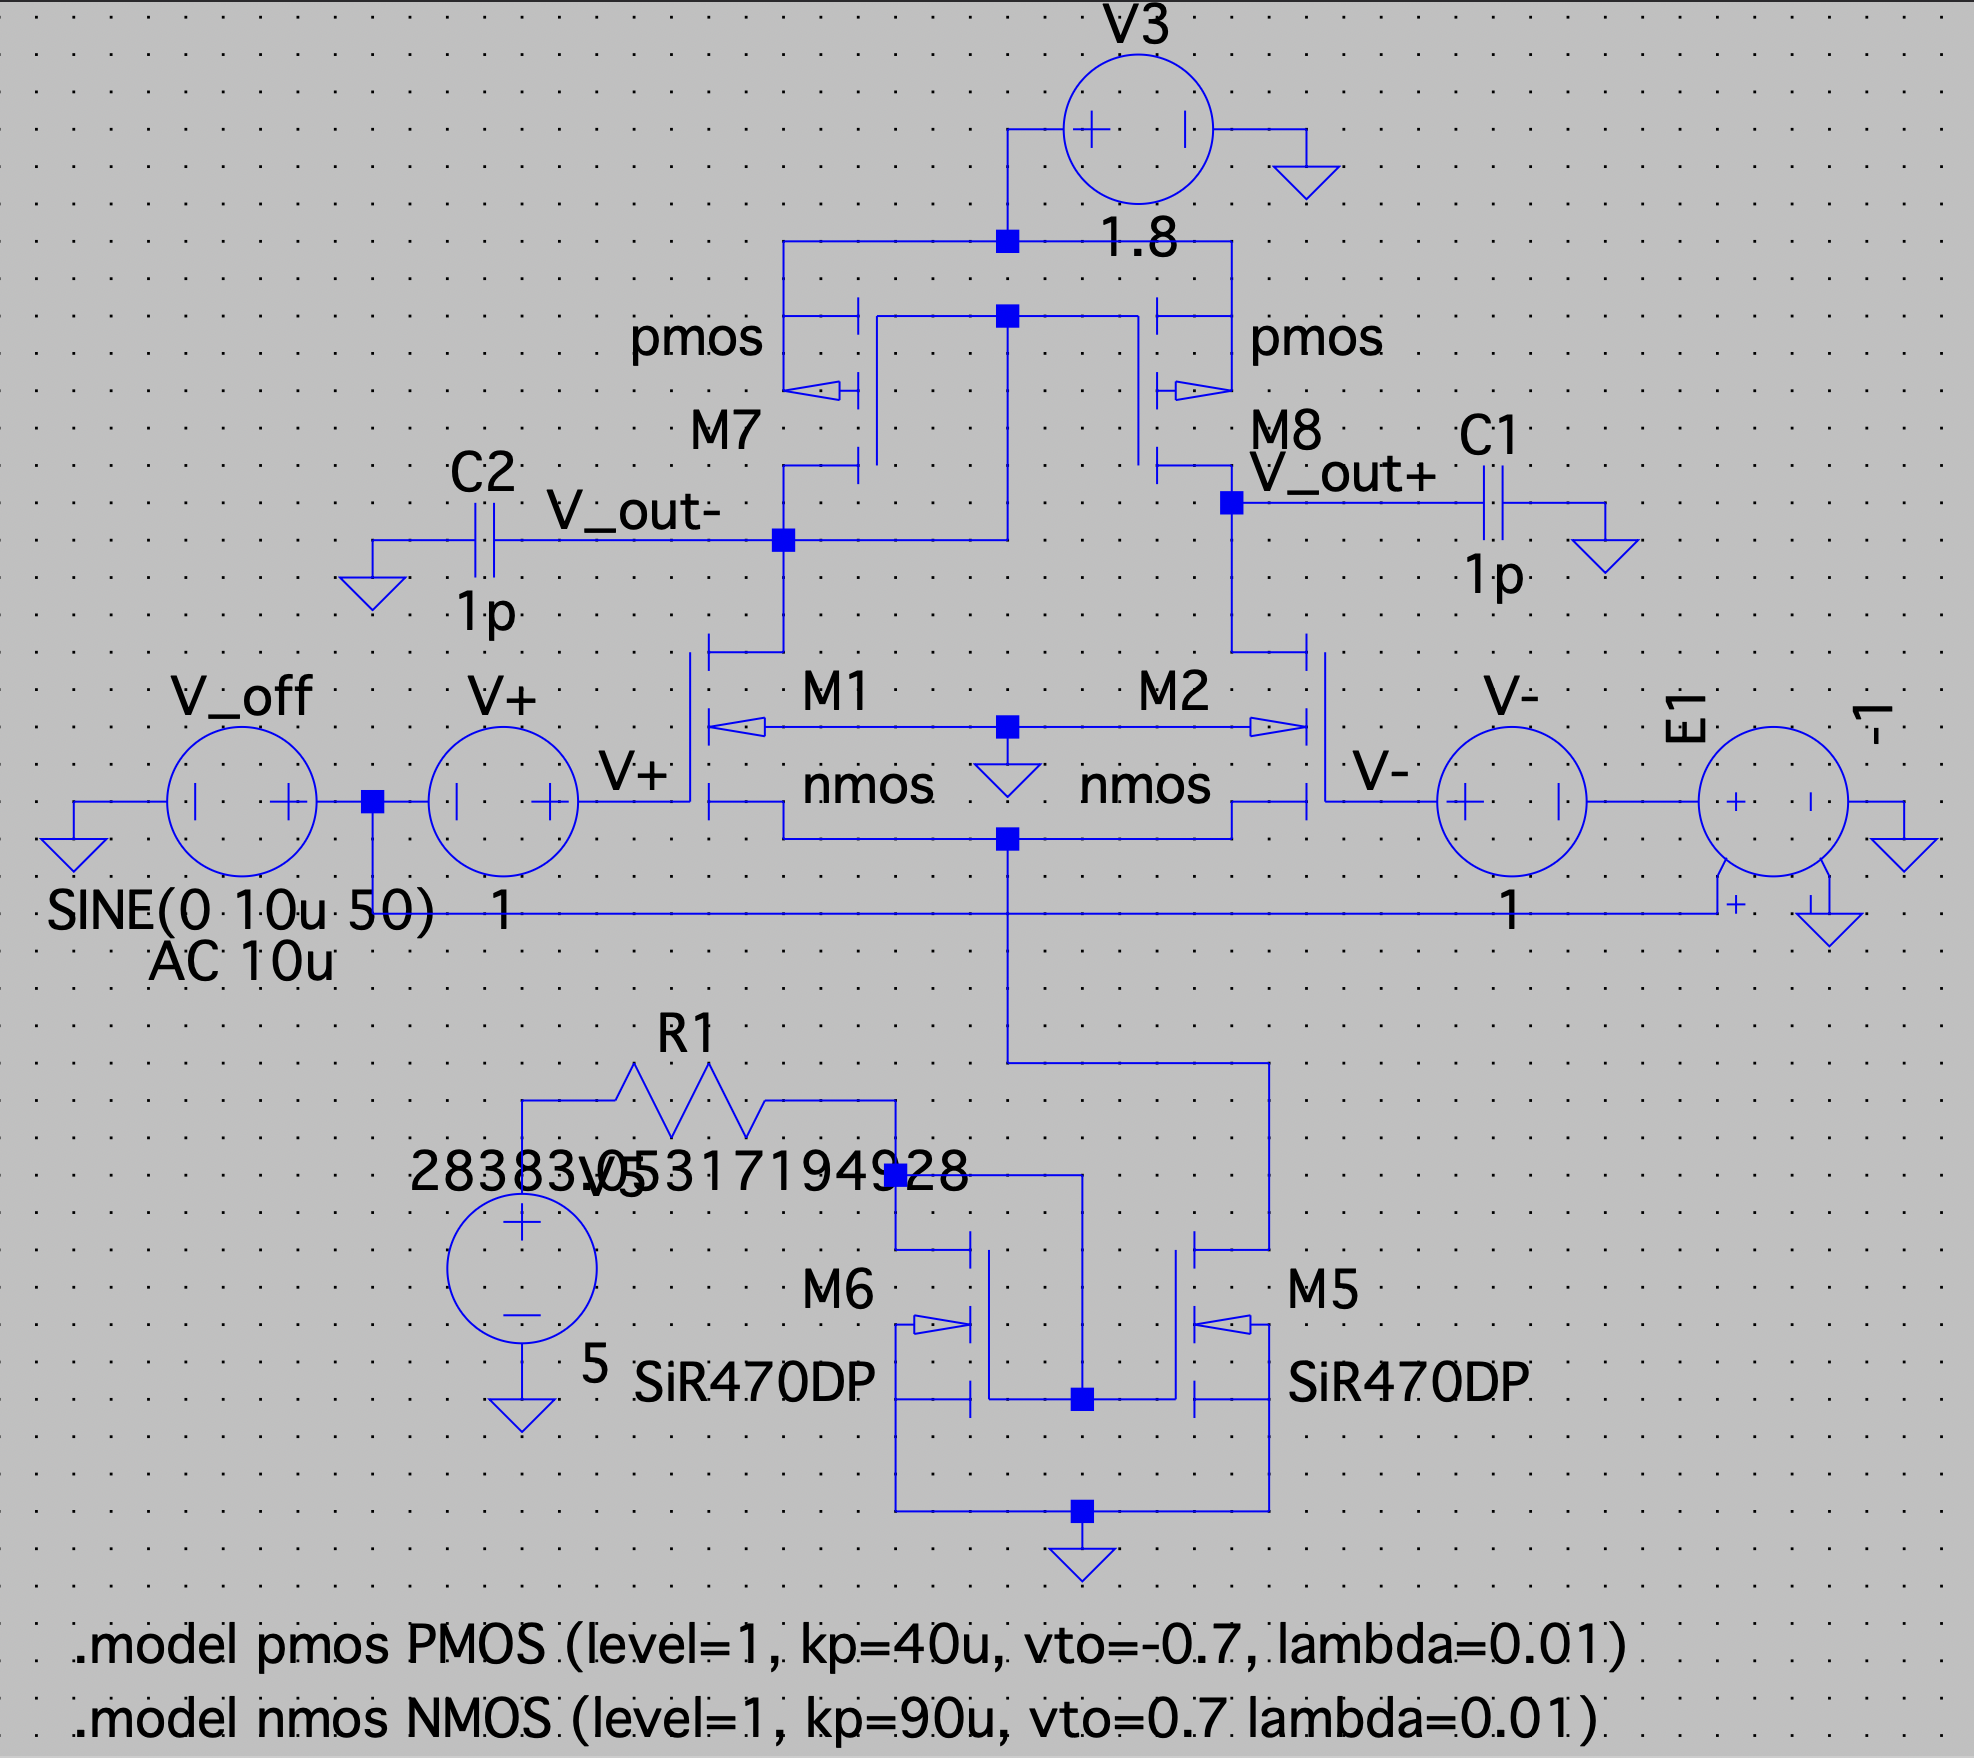
\includegraphics[width=0.8\textwidth]{figs/ckt.png}
\end{figure}
We can analyze each section seperately,
\subsection{Current Mirror}
\begin{figure}[ht!]
	\centering
	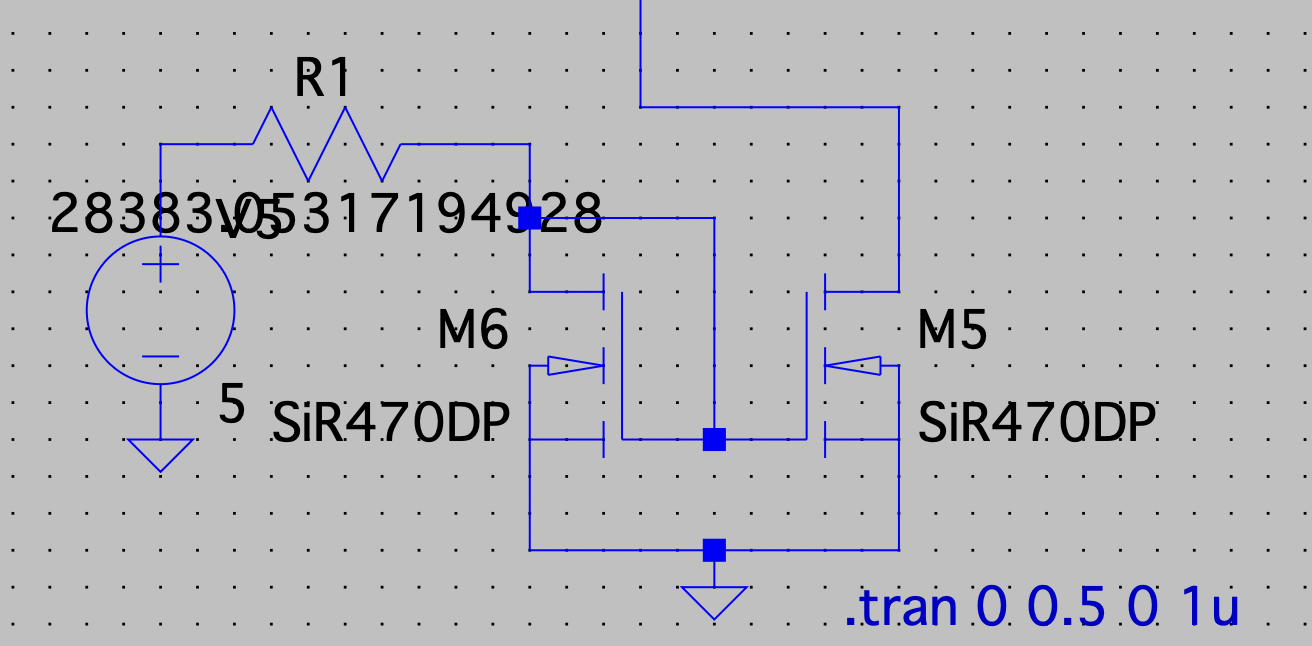
\includegraphics[width=0.8\textwidth]{Simluations/Experiment_4/figs/current_mirror.png}
\end{figure}
\pagebreak
\subsection{PMOS Active load}
\begin{figure}[ht!]
	\centering
	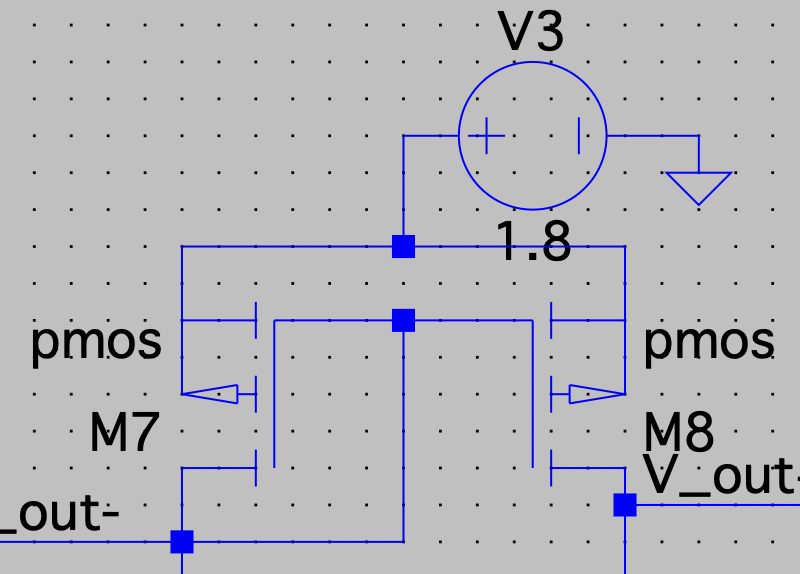
\includegraphics[width=0.8\textwidth]{Simluations/Experiment_4/figs/active_load.png}
\end{figure}
\subsection{Input NMOS}
\begin{figure}[ht!]
	\centering
	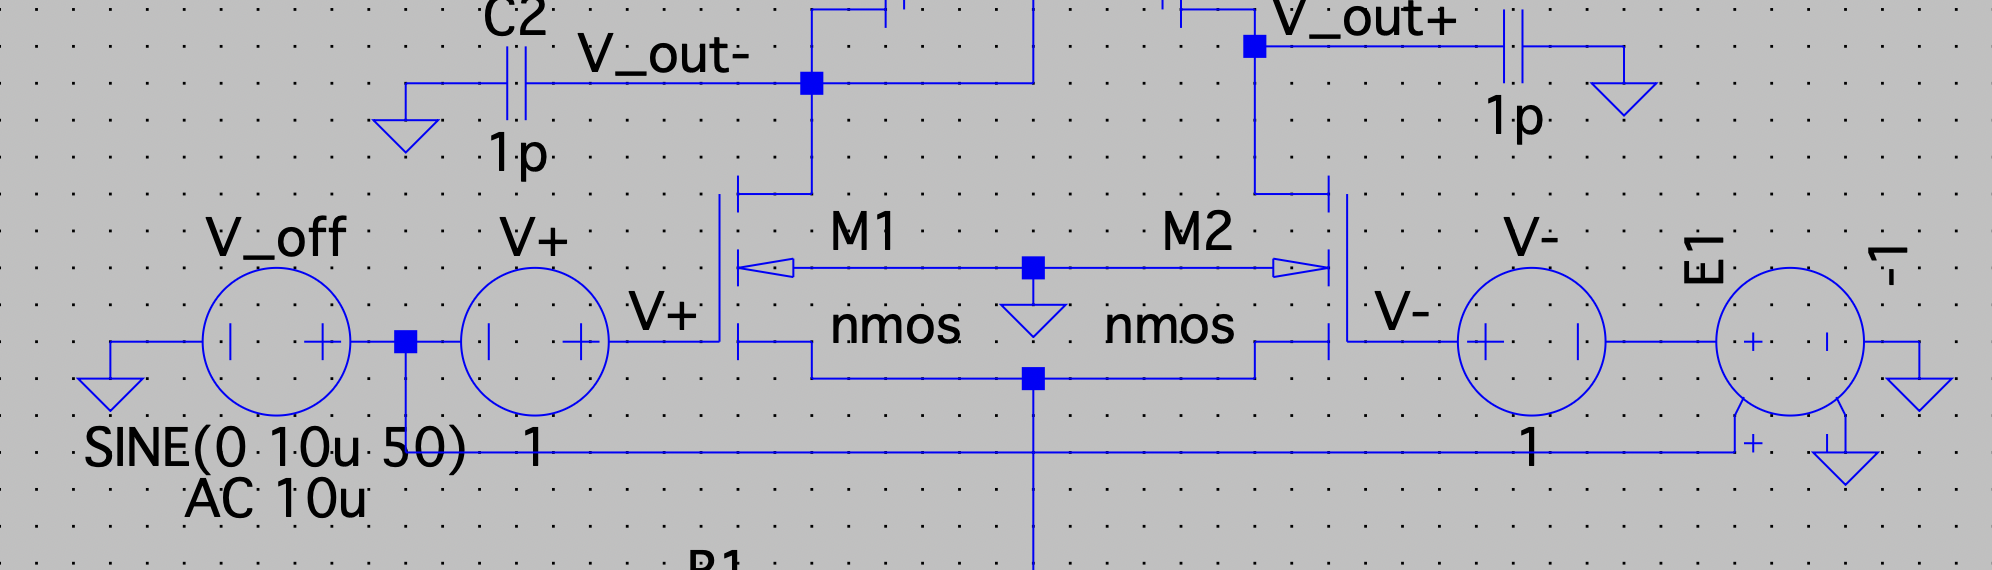
\includegraphics[width=0.8\textwidth]{Simluations/Experiment_4/figs/input_nmos.png}
\end{figure}
\subsection{MOSFET Parameters}
\begin{figure}[ht!]
	\centering
	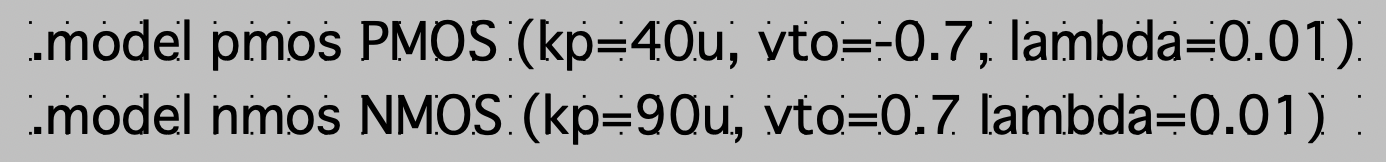
\includegraphics[width=0.8\textwidth]{Simluations/Experiment_4/figs/param.png}
\end{figure}
For PMOS, $\mathbf{W=100\mu m}$, $\mathbf{L=1\mu m}$ and NMOS $\mathbf{W=50\mu m}$, $\mathbf{L=1\mu m}$. For the MOSFETs used in current mirror, $\mathbf{kp=69.6391, V_{to}=2.16V}$.
\vspace{10pt}
\pagebreak
\section{DC OP point}
Current obtained through current mirror can be adjusted through adjusting the $R$ value. It is done by solving the equations,
\begin{align*}
    I = 100\mu A = \frac{V_S-V_D}{R} = \frac{k_p}{2}(V_{GS}-2.16)^2
\end{align*}
\begin{figure}[H]
    \centering
    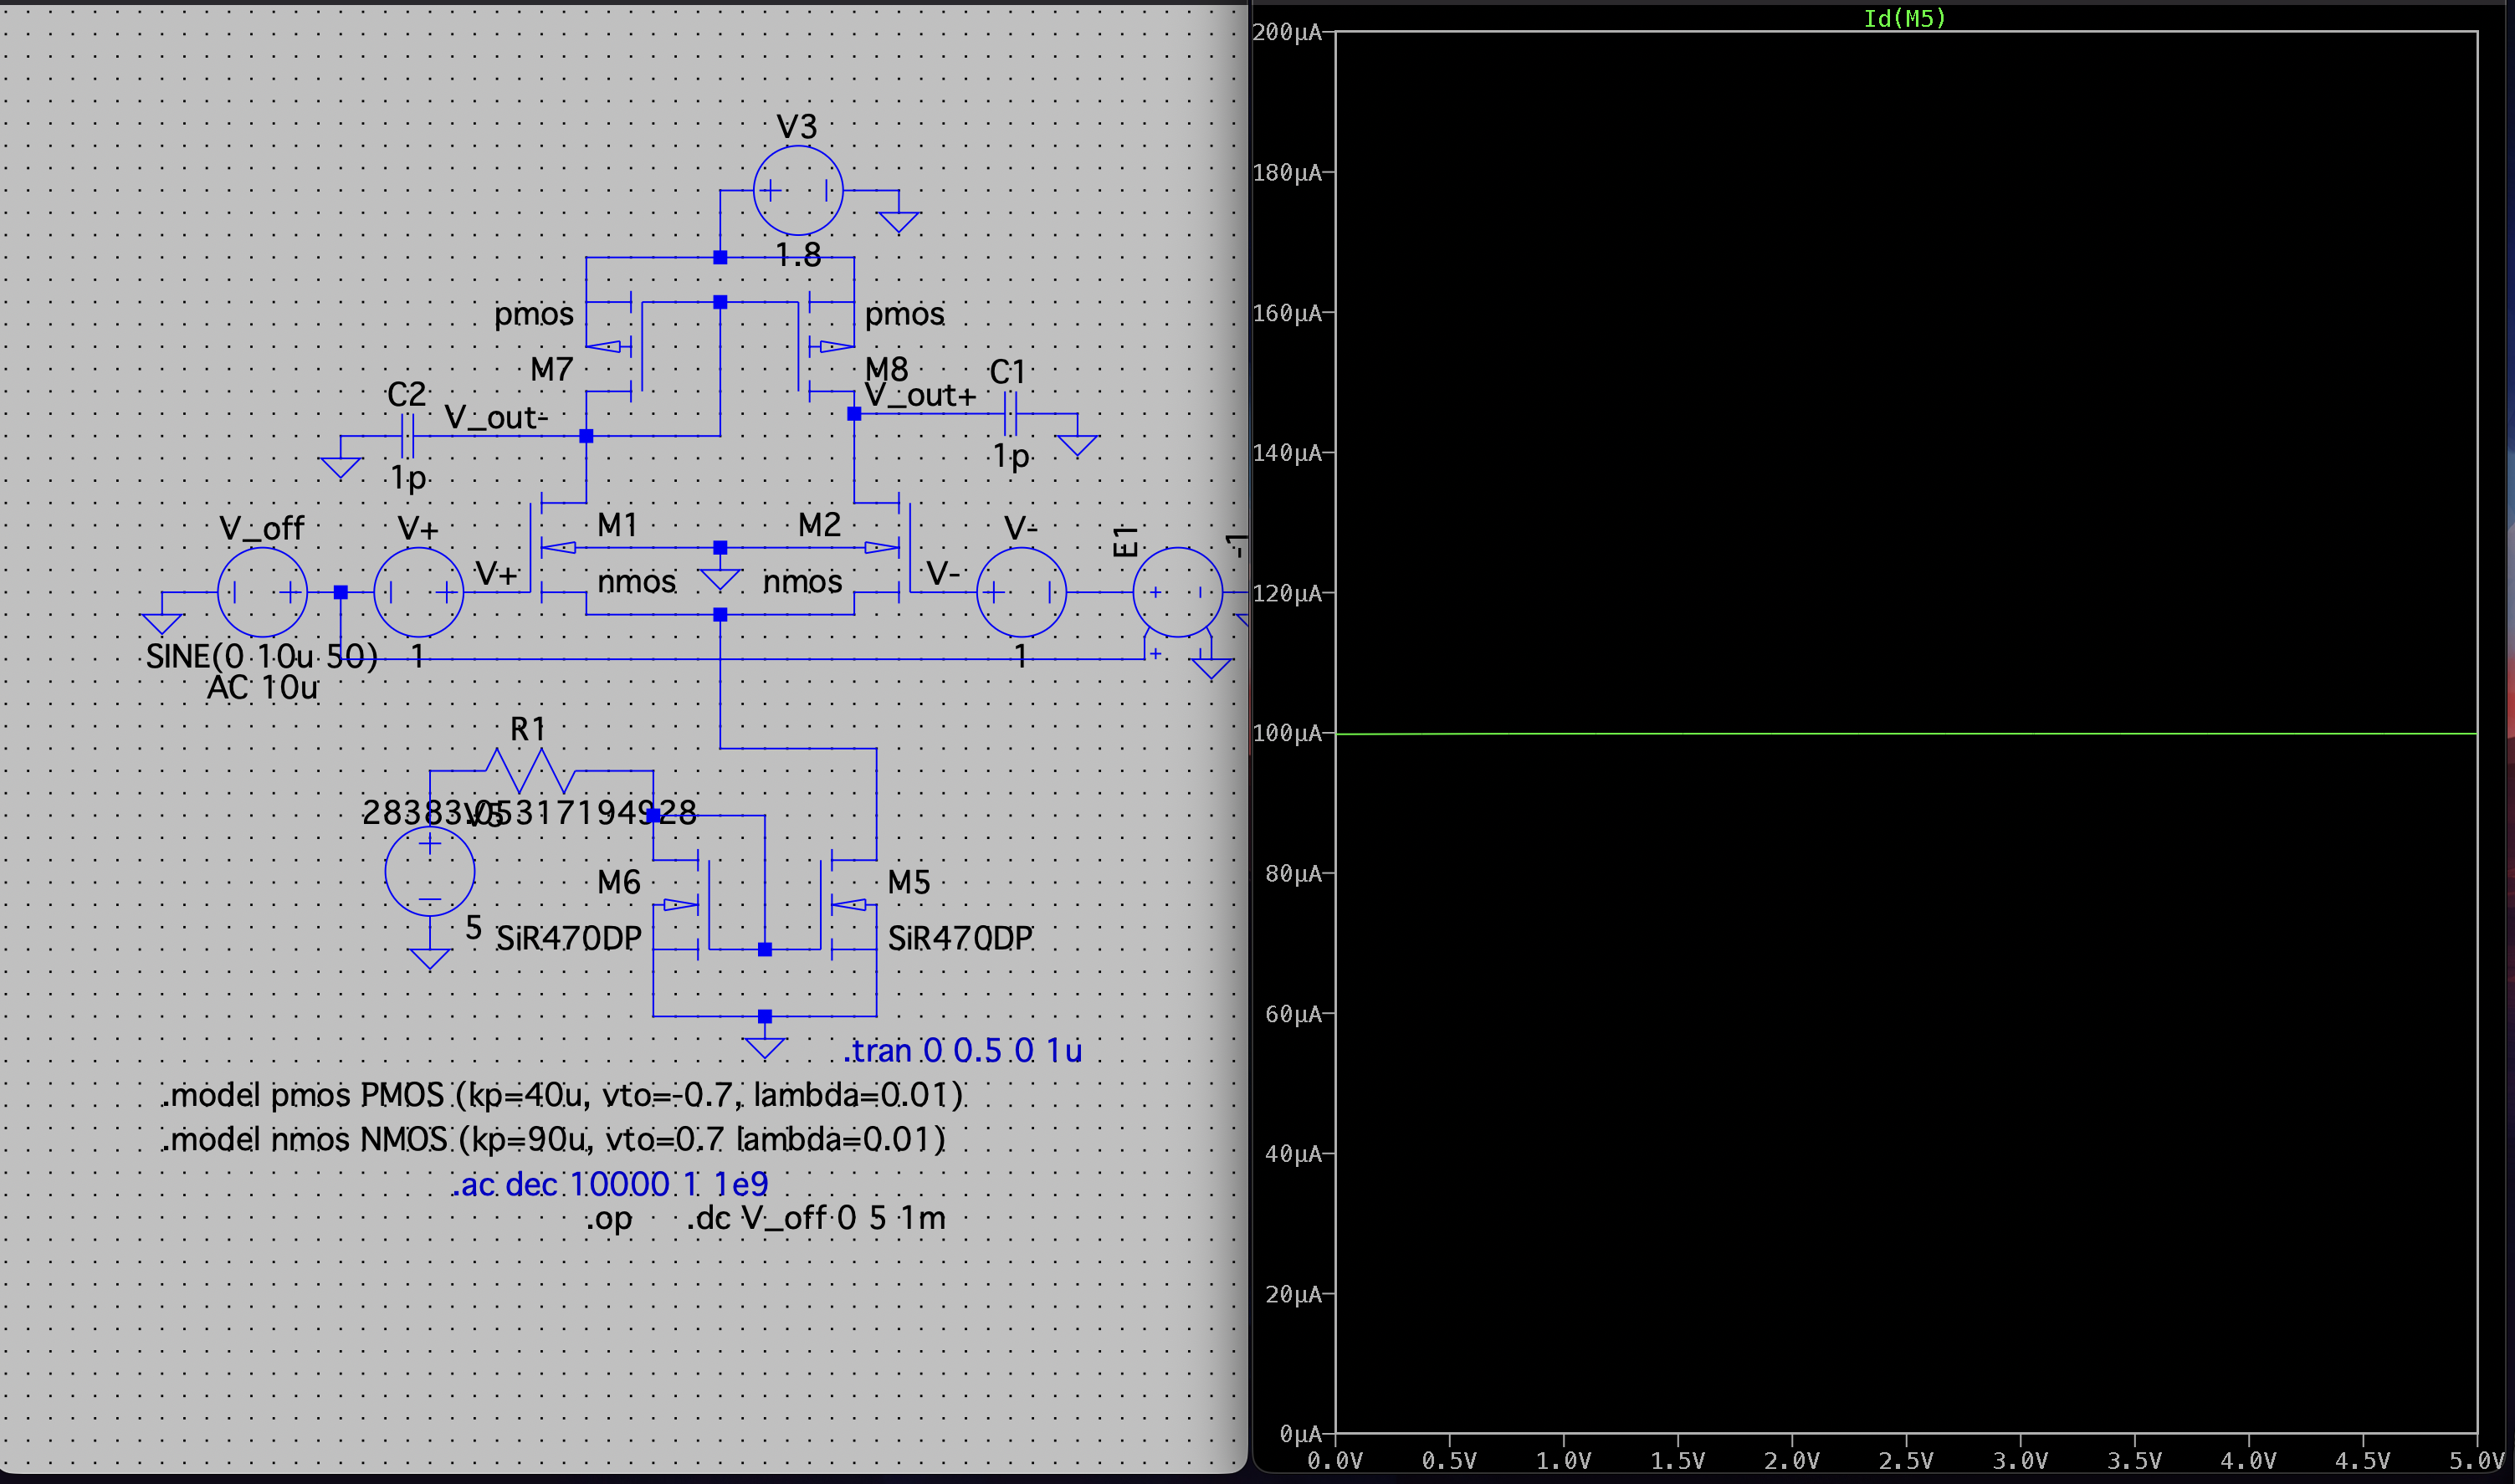
\includegraphics[width=0.8\textwidth]{Simluations/Experiment_4/figs/current.png}
\end{figure}
We have to choose $V_+, V_-$ values such that MOSFETs M1 and M2 are in saturation. We do so by plotting $V_{DS}$ vs $V_{GS}-V_{TO}$ and choose $V_+$ appropriately,
\begin{figure}[H]
    \centering
    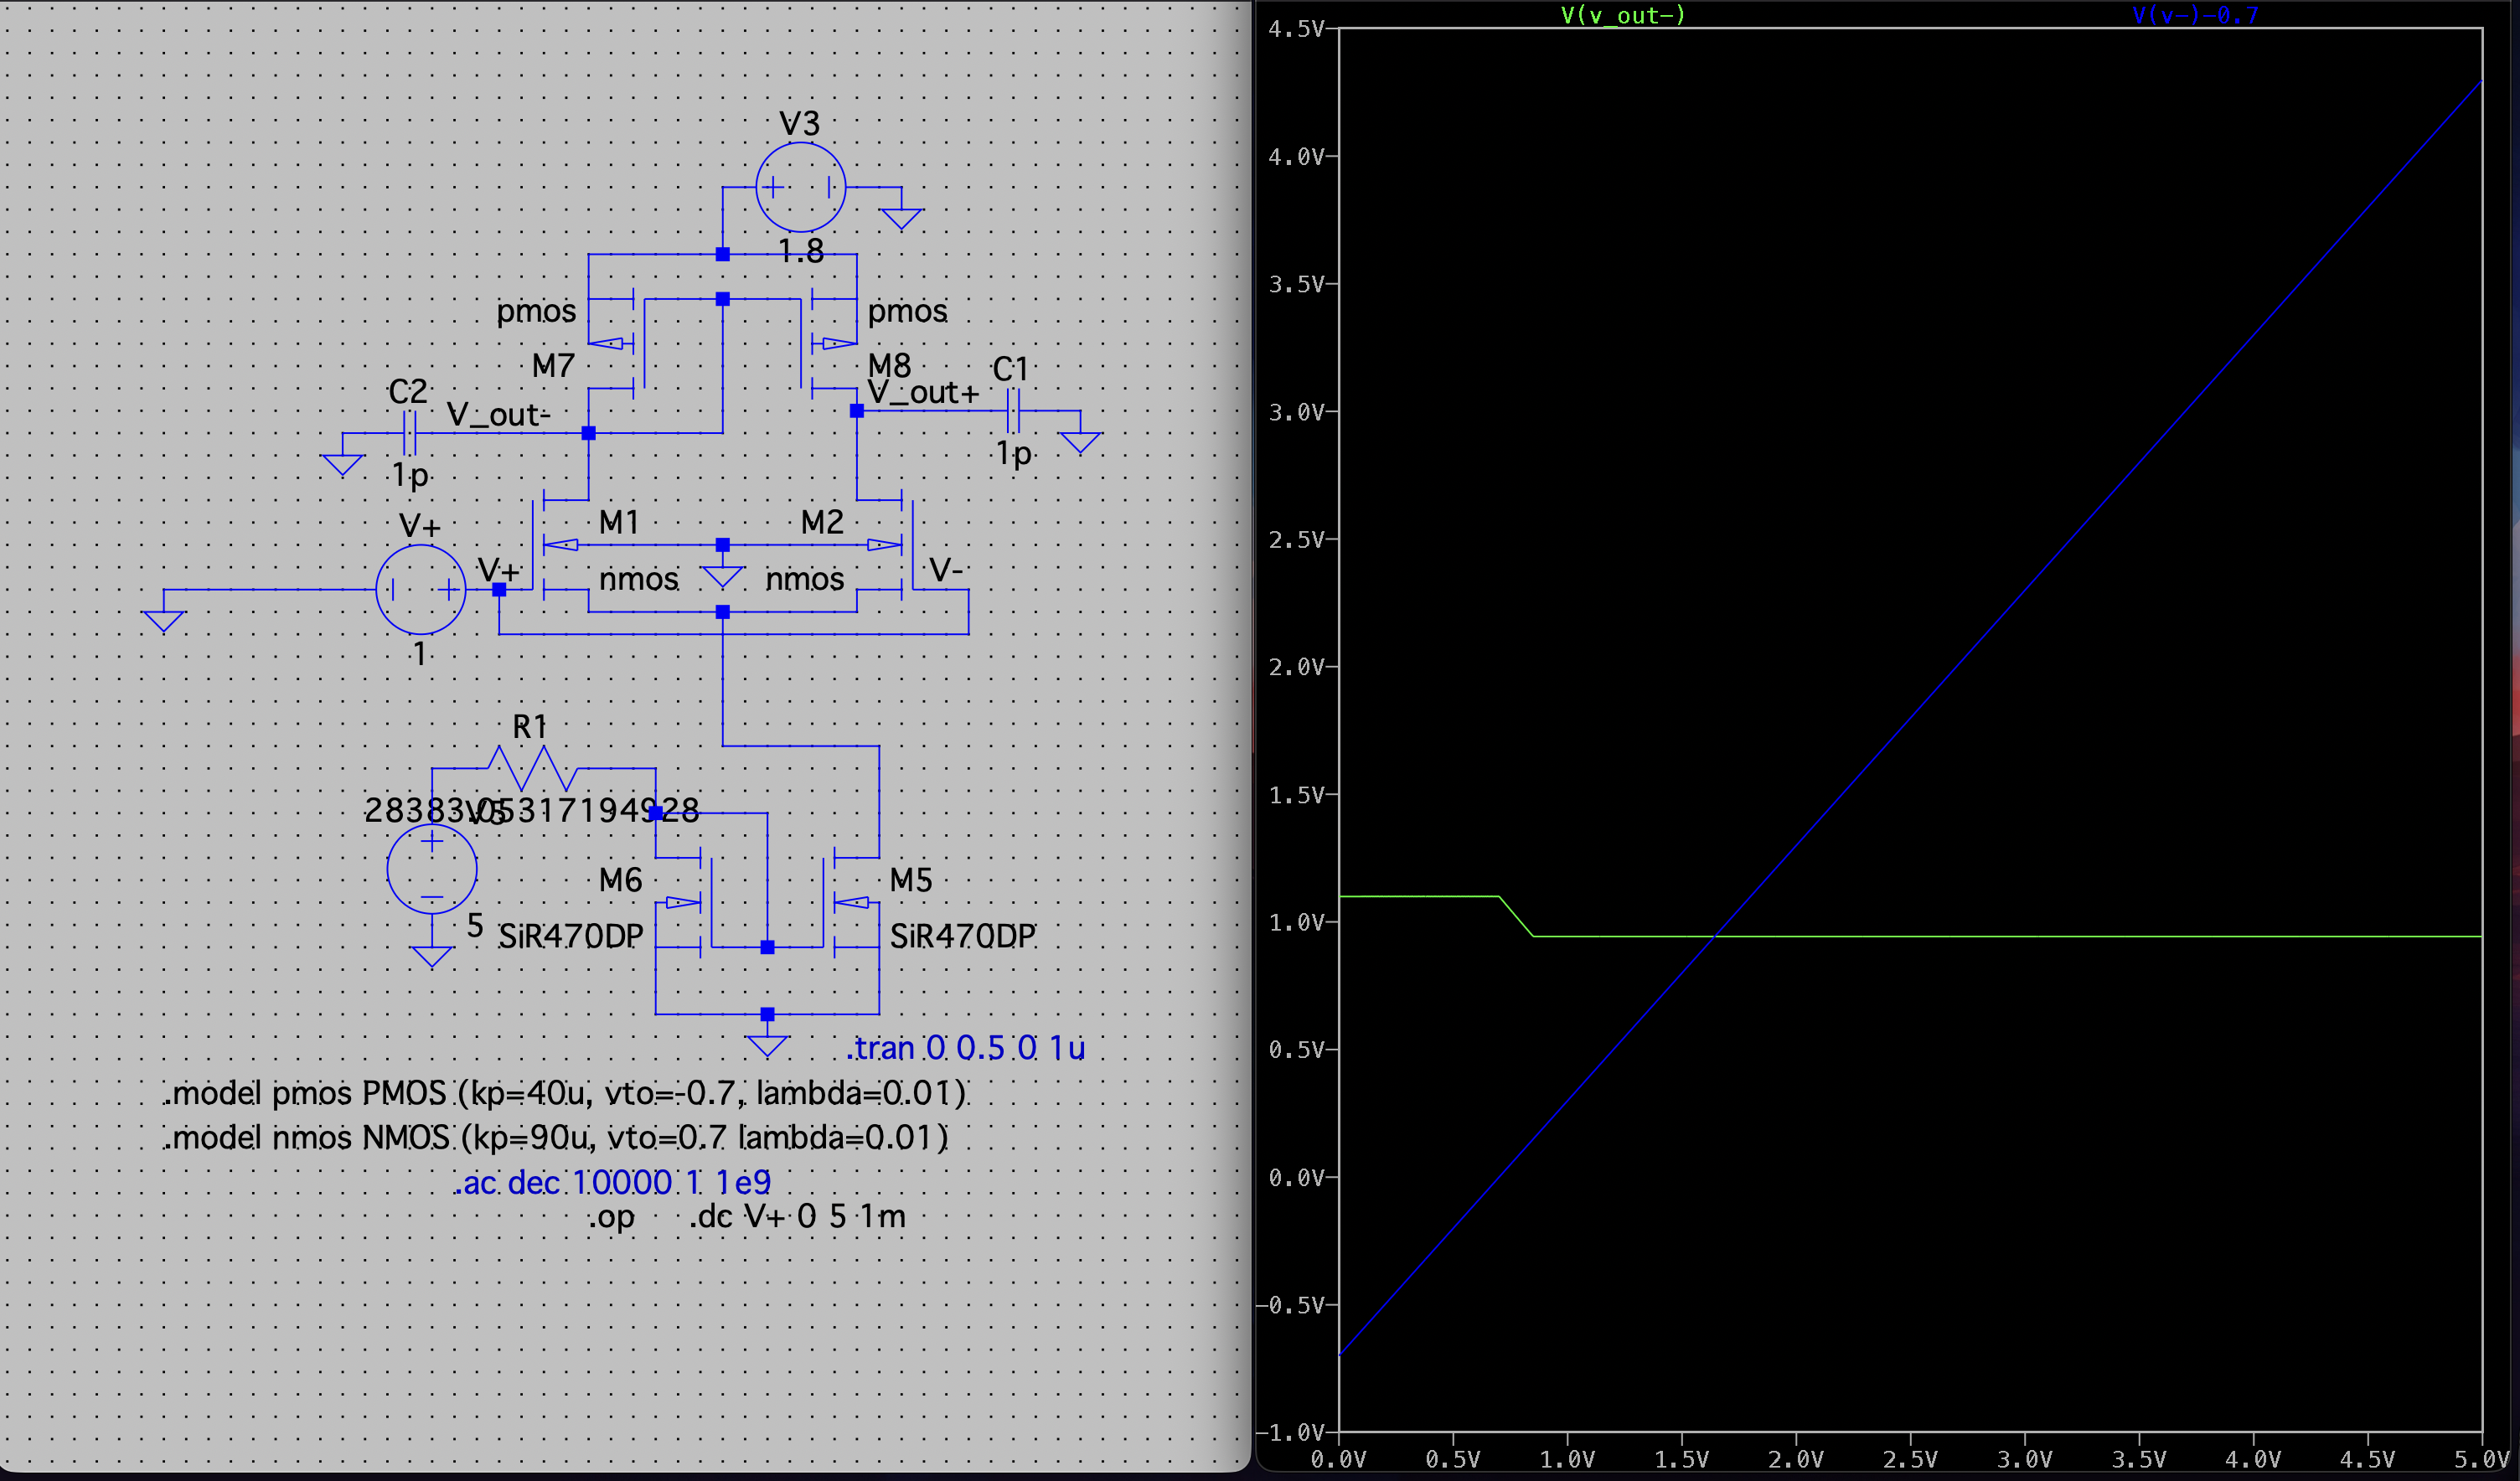
\includegraphics[width=0.8\textwidth]{Simluations/Experiment_4/figs/saturation_1.png}
\end{figure}
We choose bias point to be $1V$ so that MOSFETs M1 and M2 are comfortably in saturation.
\begin{figure}[H]
    \centering
    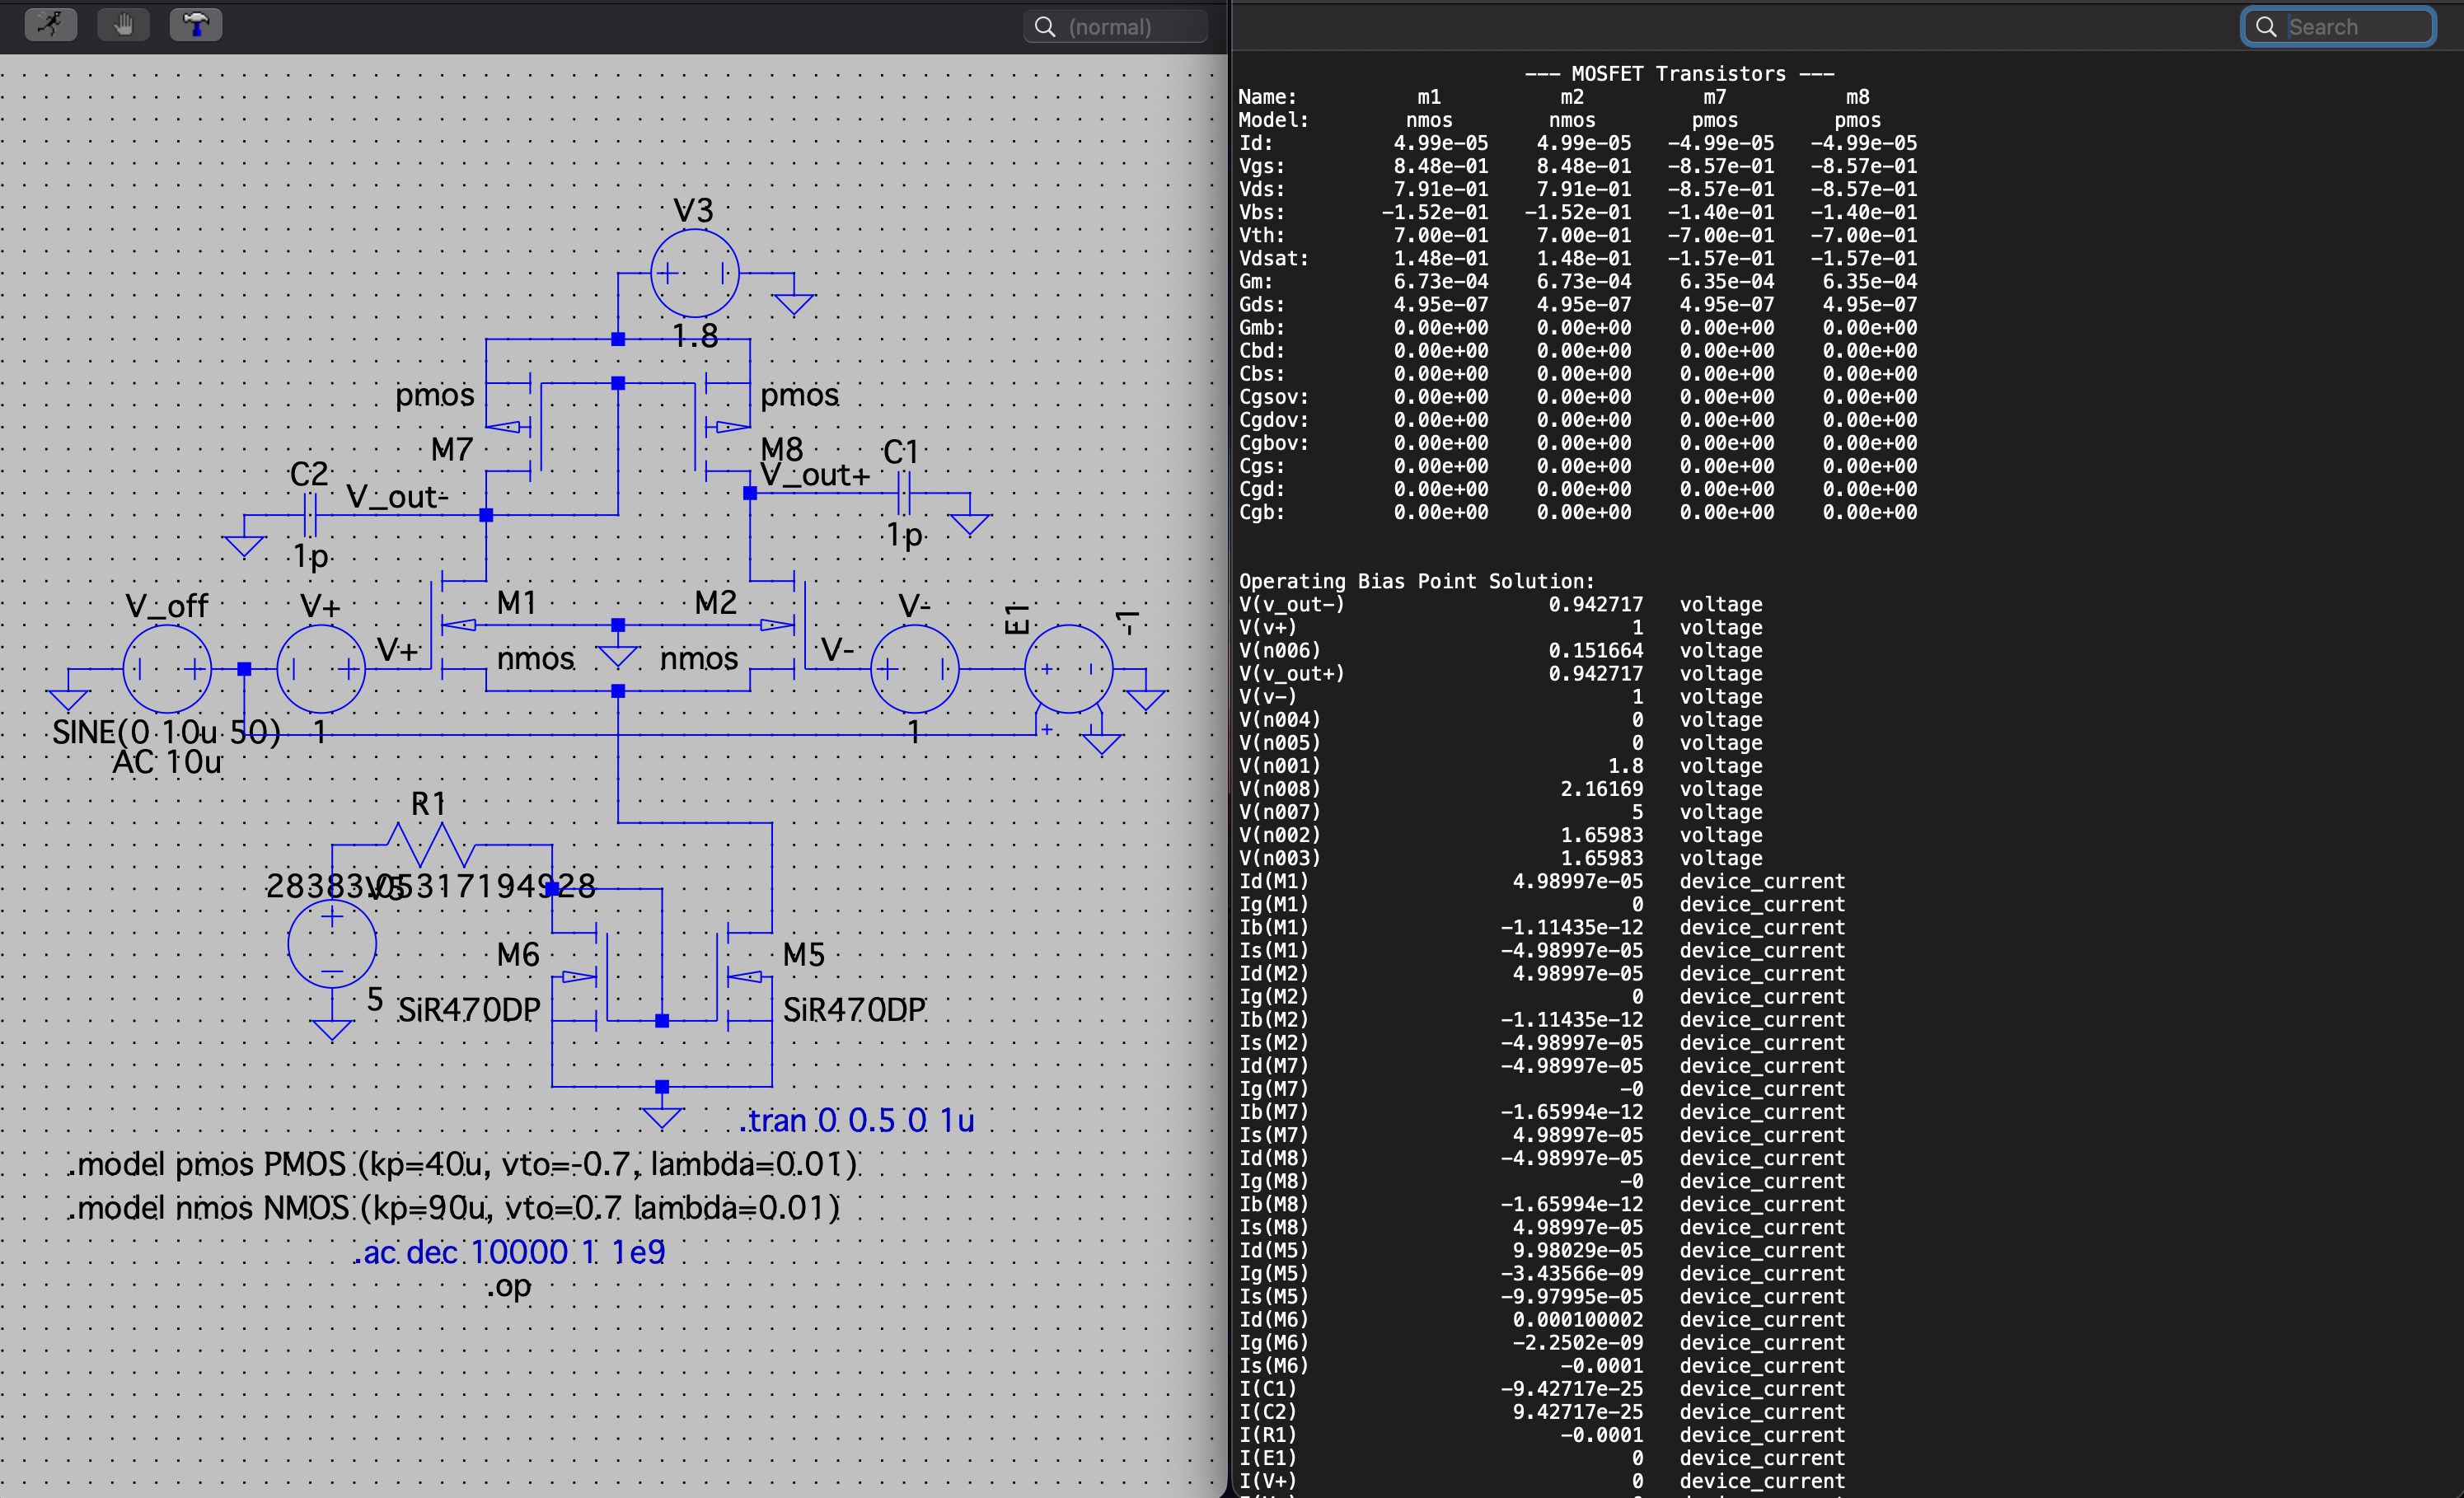
\includegraphics[width=0.8\textwidth]{figs/op.png}
\end{figure}
\vspace{6pt}
\section{Differential Gain}
Small signal parameters of MOSFETs are given by,
\begin{align*}
    g_m &= \frac{2I_D}{V_{GS}-V_{TO}} = \frac{\partial I_D}{\partial V_{GS}}\\
    r_o &= \frac{1}{\lambda I_D} =  \frac{\partial V_{DS}}{\partial I_D}
\end{align*}
Differential gain is given by 
\begin{align*}
    A_d = g_{m1} (r_{o1} \parallel r_{o7}) = \frac{V_{out}}{V_{id}}
\end{align*}
Where $V_{id}=V_+-V_-$, $g_{m1}$ is transconductance of NMOS M1, $r_{o1}, r_{o7}$ are output resistances of NMOS M1 and PMOS M7 respectively.\newline
\begin{figure}[H]
    \centering
    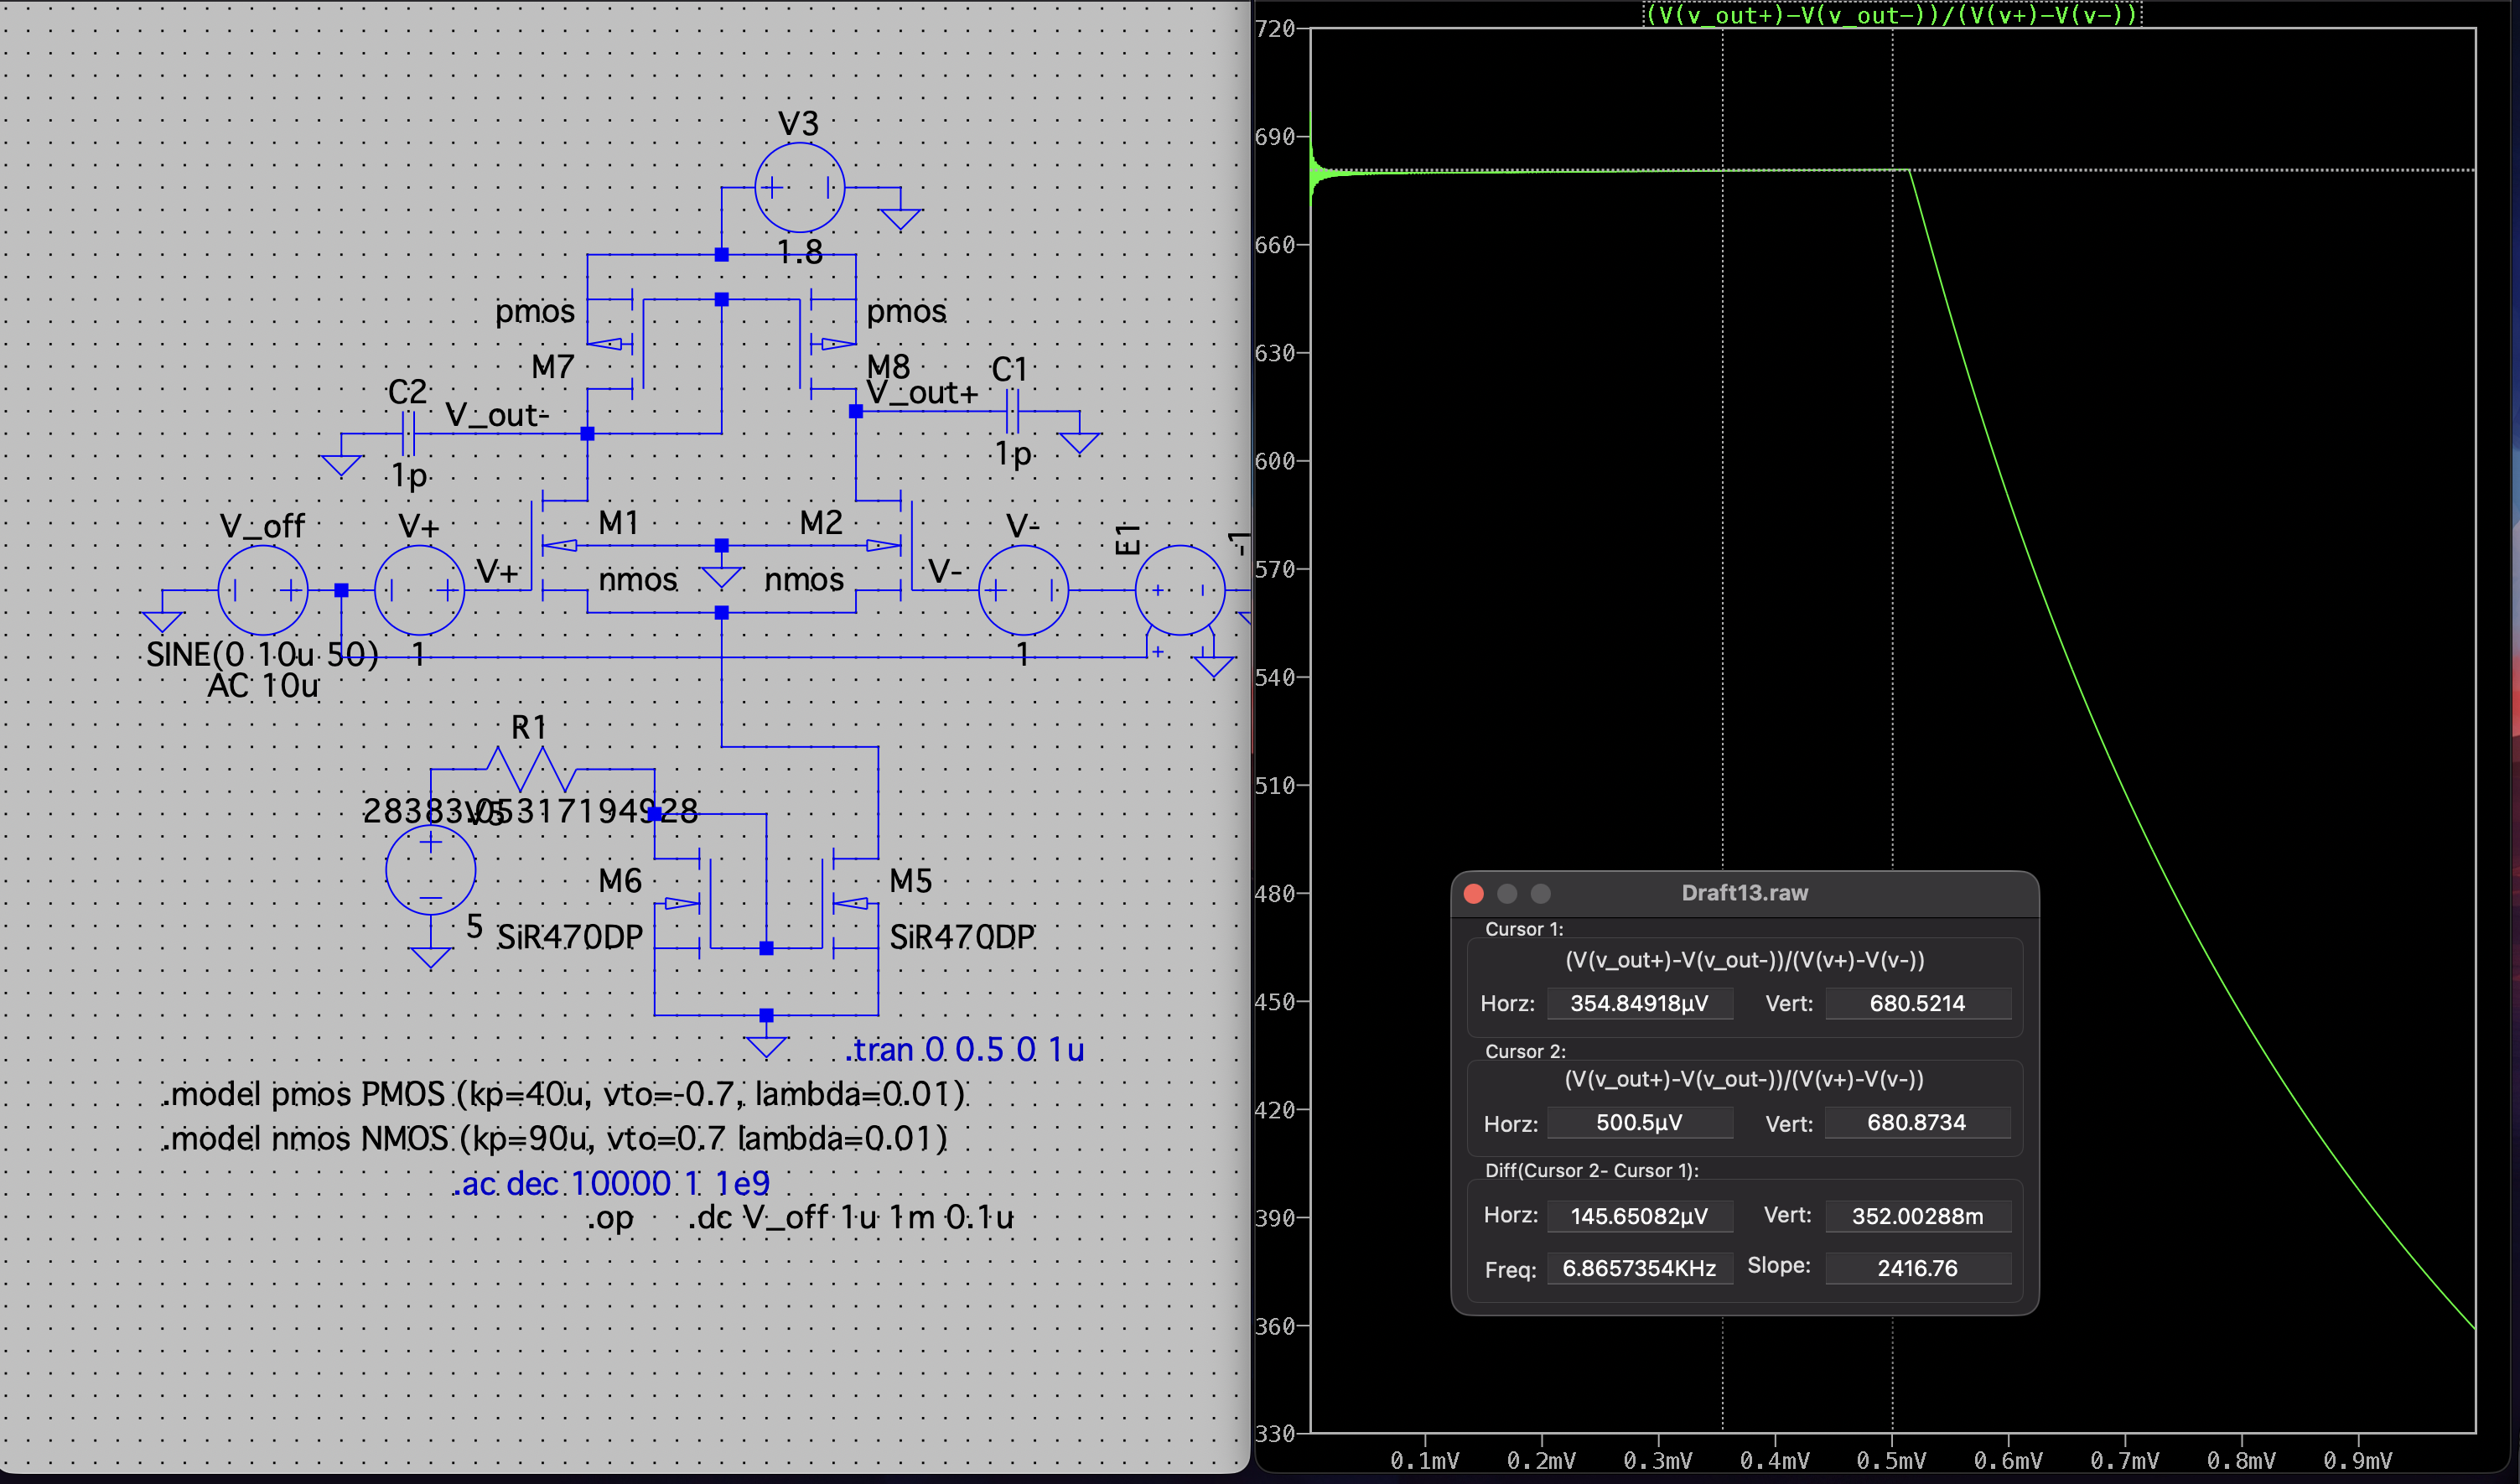
\includegraphics[width=0.8\textwidth]{figs/gain_1.png}
\end{figure}
\vspace{6pt}
\begin{figure}[H]
    \centering
    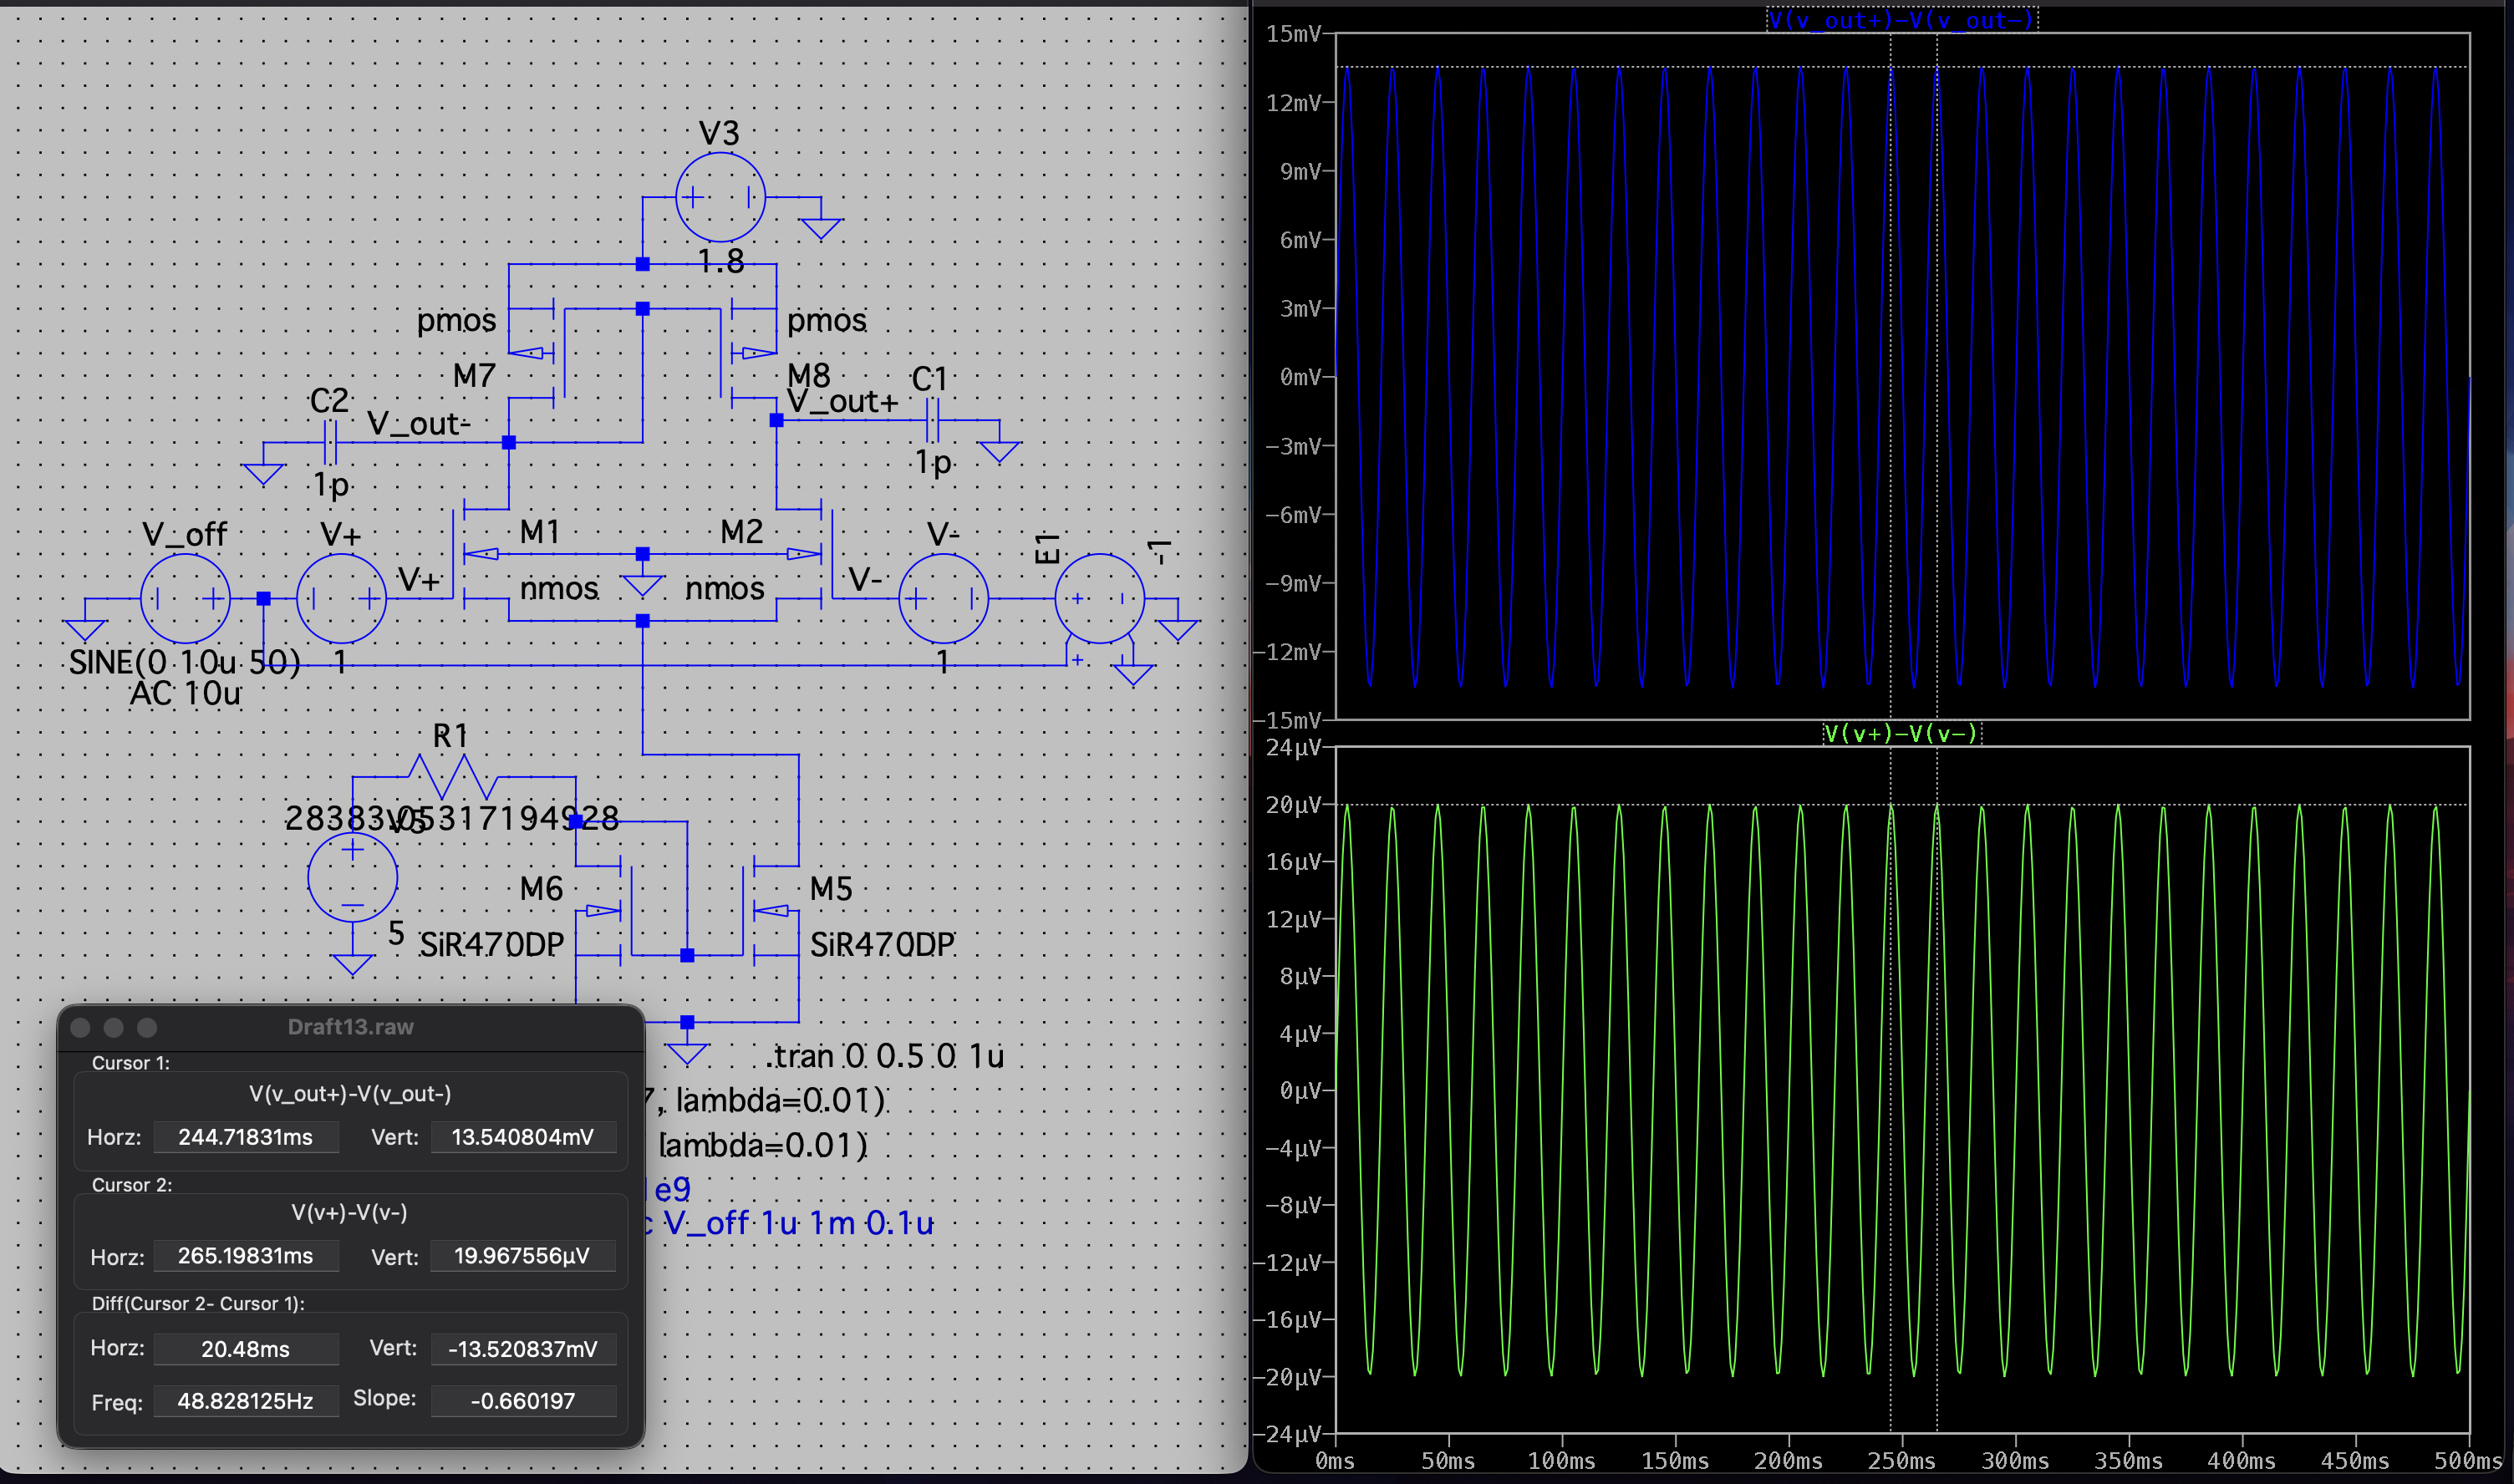
\includegraphics[width=0.8\textwidth]{figs/gain_2.png}
\end{figure}
We get,
\begin{itemize}
    \item Theoretical Gain: $674.145183906806$
    \item Observed Gain: $680.5214$
\end{itemize}
\vspace{10pt}
\section{Input-Referred Offset}

\section{Common-Mode Rejection Ratio (CMRR)}
\textbf{Theory:}
\begin{align*}
\textbf{CMRR} = 20 \log{\brak{\frac{A_{d}}{A_{cm}}} }
\end{align*}
where $A_{cm}$ is the common-mode gain,
\begin{align*}
    A_d &= \frac{V_{out}}{I_D} = g_{m1}(r_{o1}\parallel r_{o7}) \\
    A_{cm} &= \frac{V_{out}}{V_{cm}} \approx \frac{g_{m1}(r_{o1}\parallel r_{o7})}{1+2g_{m1}r_{tail}} \\
    r_{tail} &= r_{o6}\parallel r_{o5}
\end{align*}
\begin{align*}
    \mathbf{CMRR \approx 2g_{m1}r_{tail}}
\end{align*}
\vspace{6pt}
\begin{figure}[H]
    \centering
    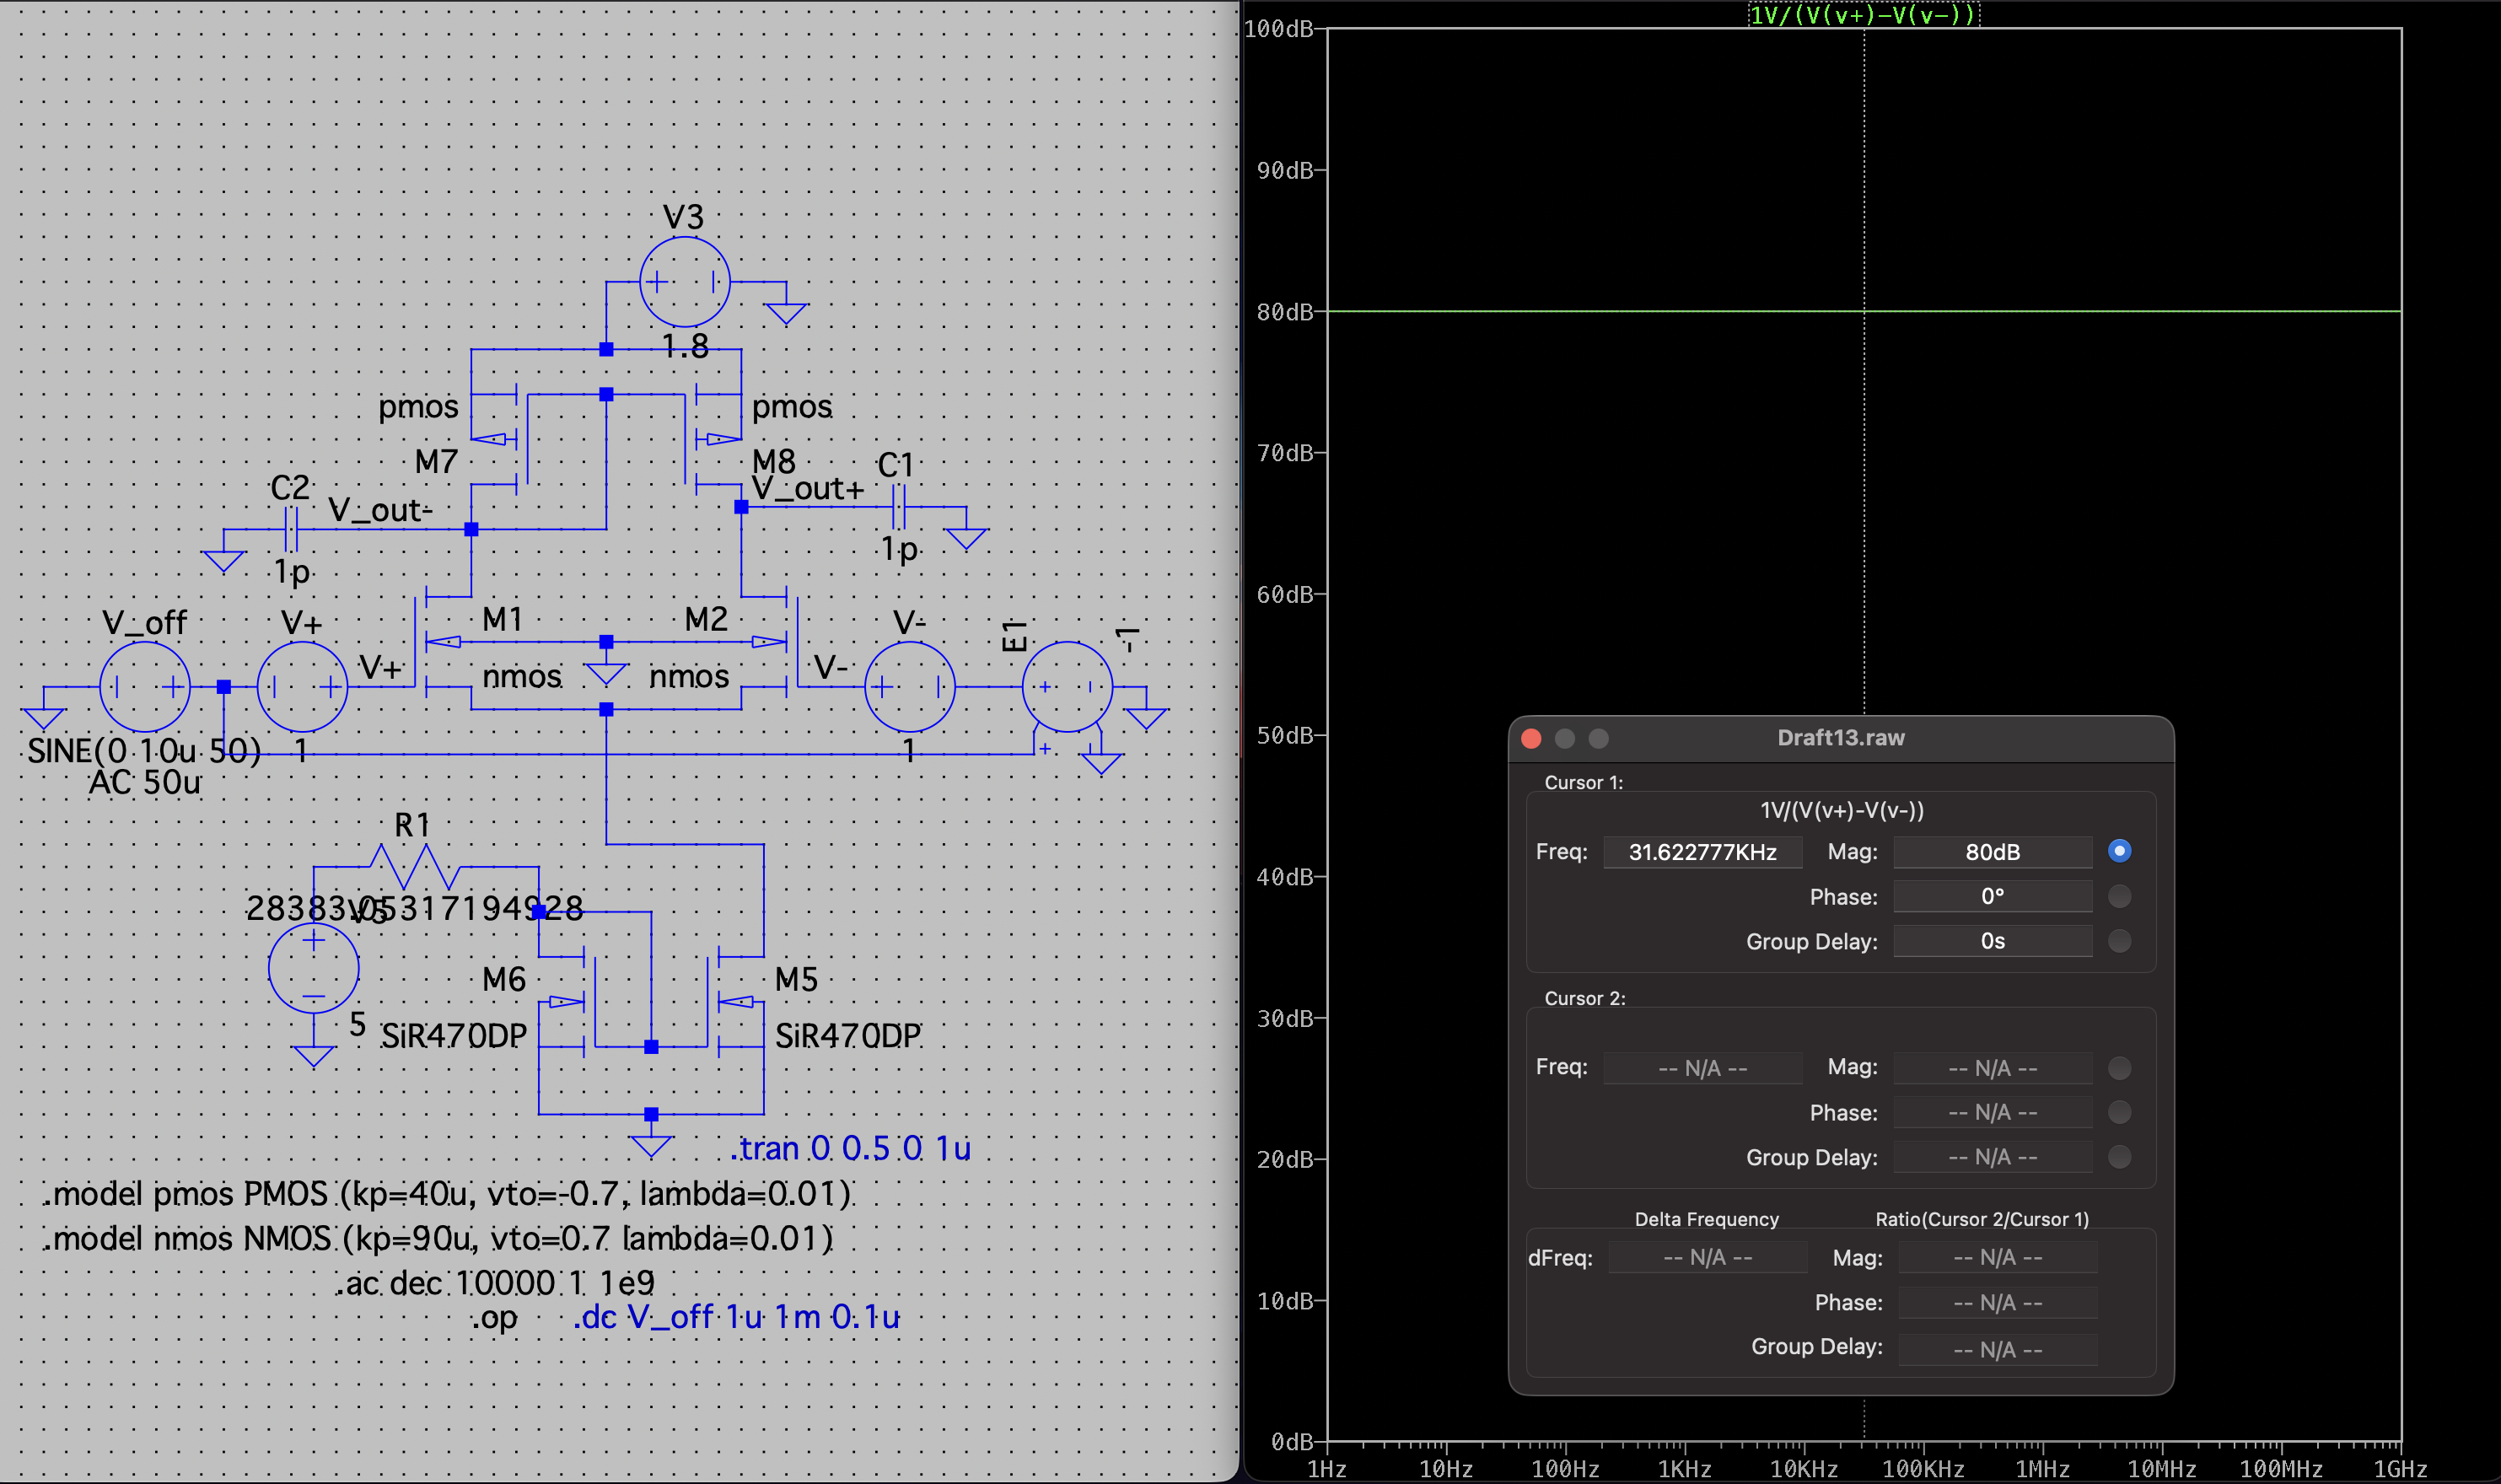
\includegraphics[width=0.8\textwidth]{figs/CMRR.png}
\end{figure}
We get,
\begin{itemize}
    \item Theoretical CMRR: $76.56610455194526 dB$
    \item Observed CMRR: $80 dB$
\end{itemize}

\vspace{10pt}
\section{Transconductance ($g_m$)}
\begin{align*}
g_m = \frac{\partial I_D}{\partial V_{GS}}= \frac{2I_D}{V_{GS}-V_{TO}}
\end{align*}
\vspace{6pt}
\begin{figure}[H]
    \centering
    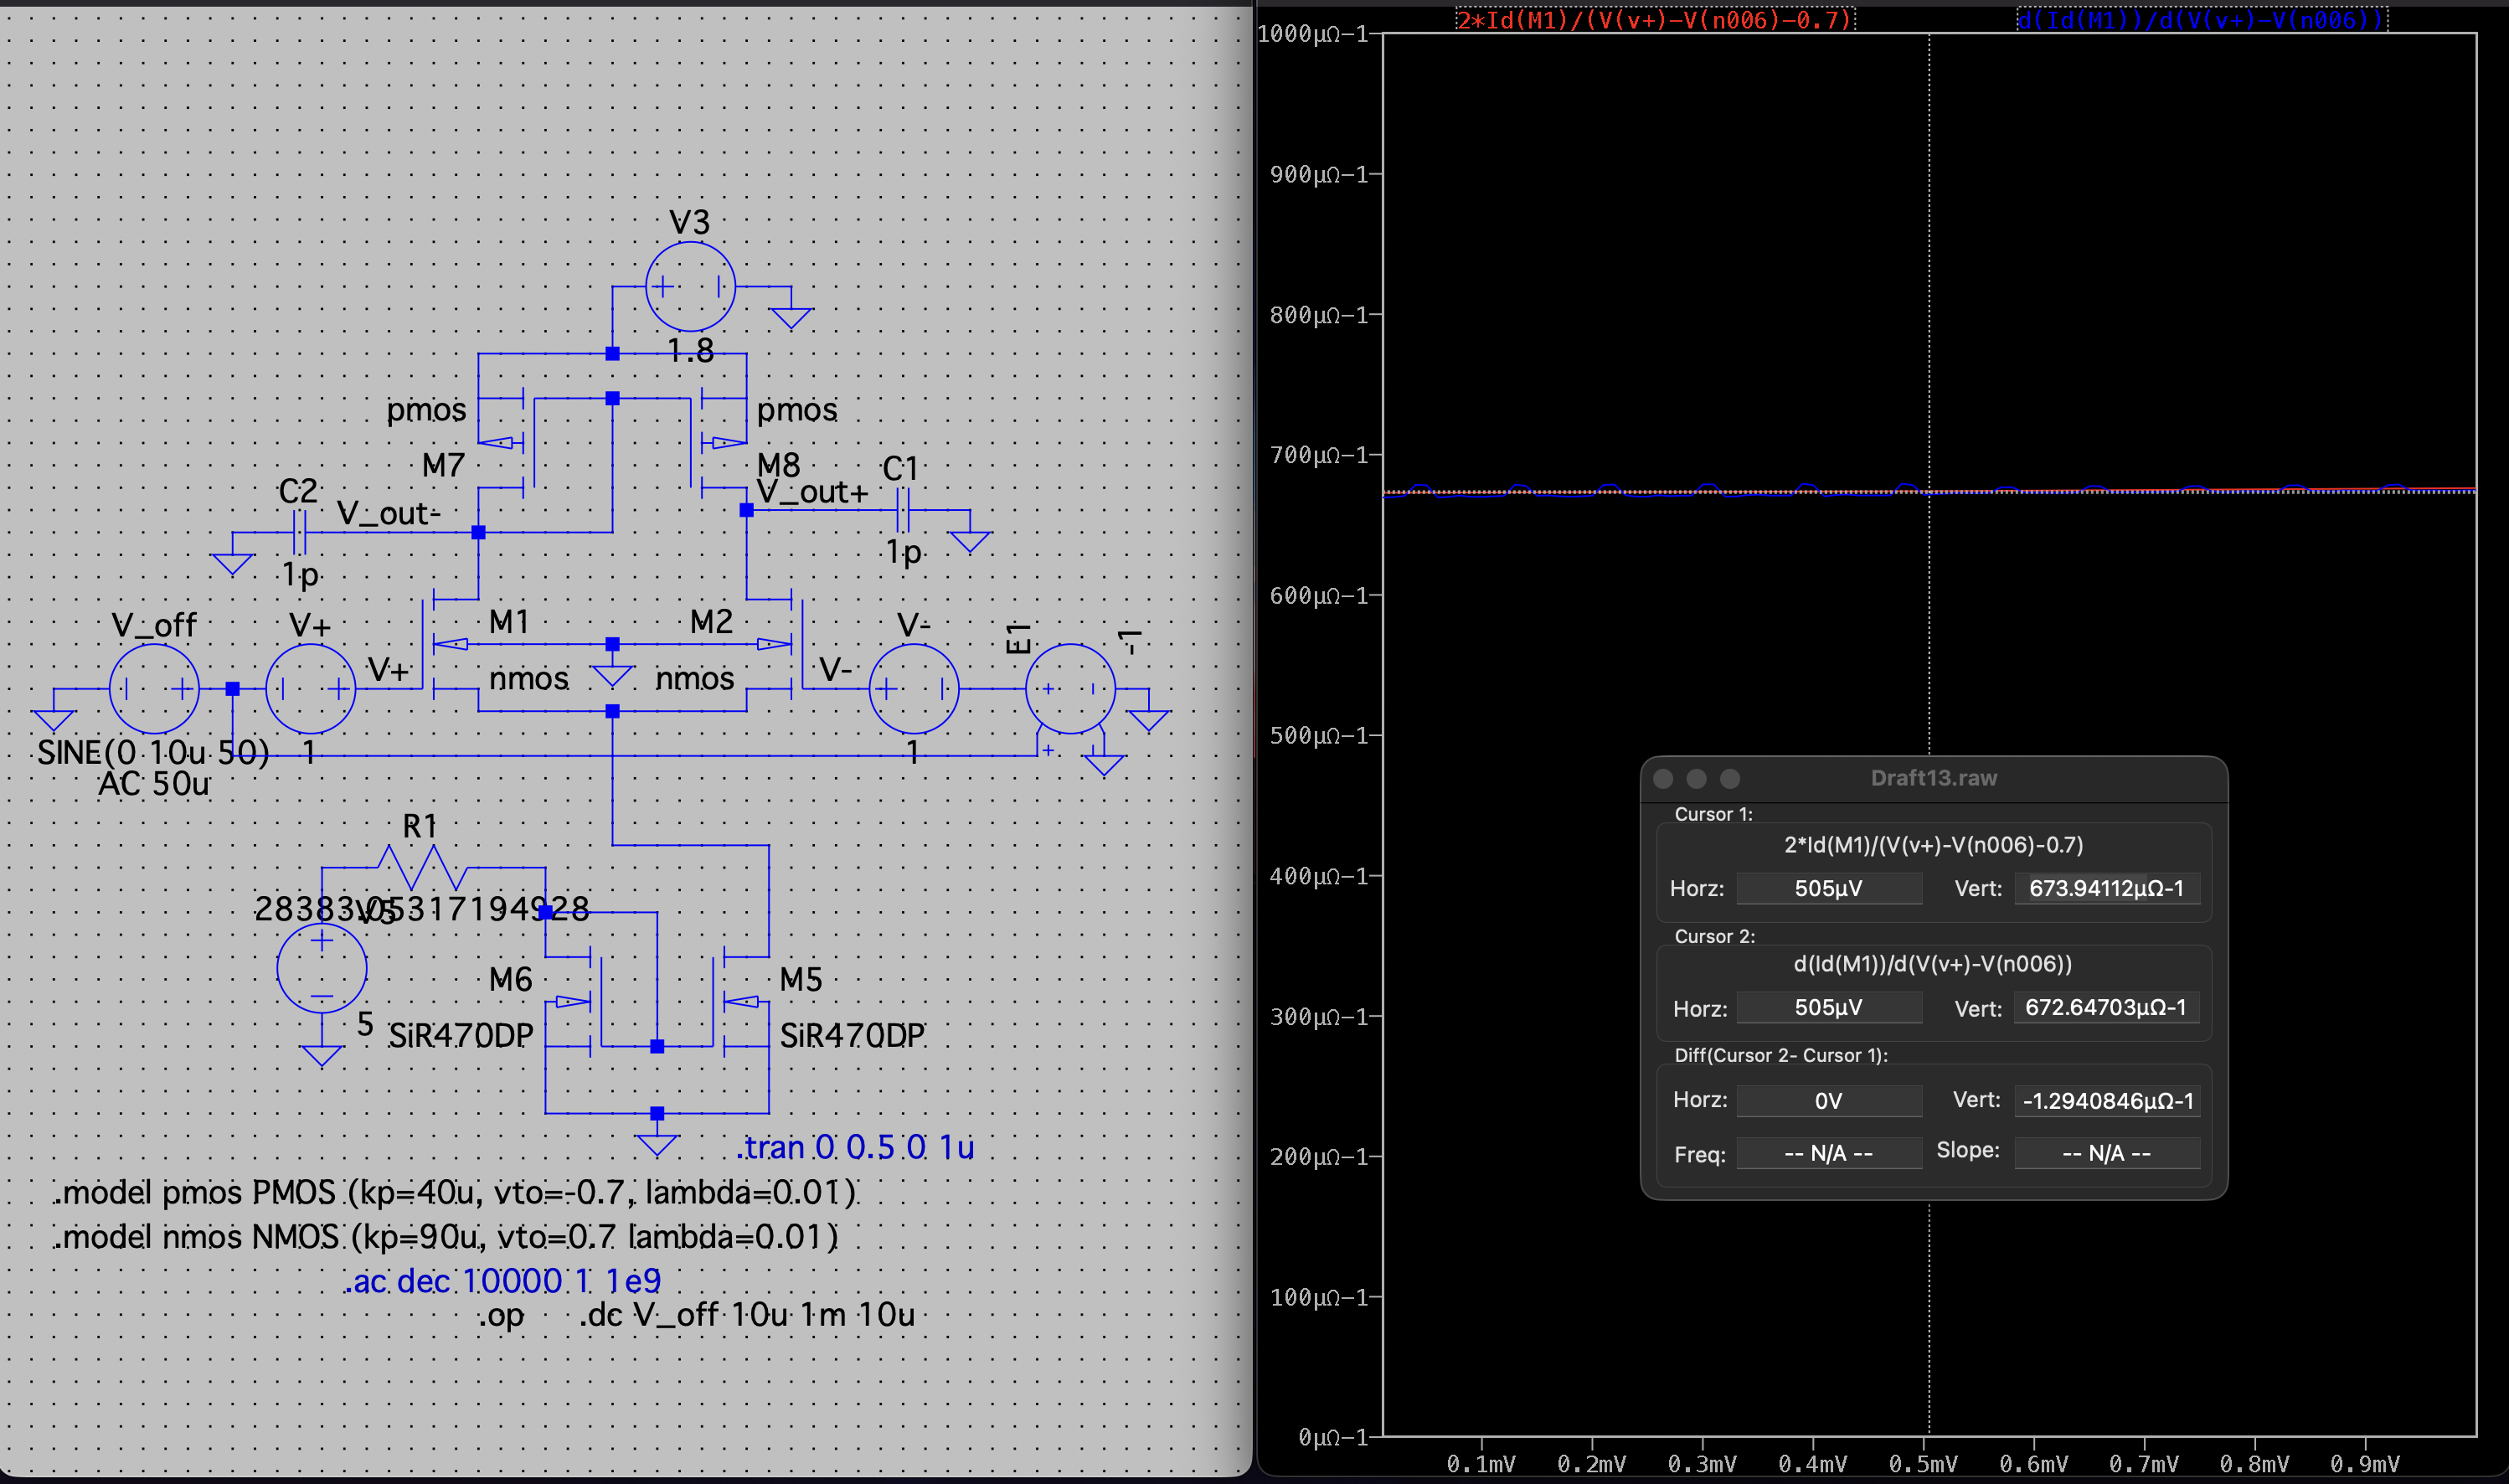
\includegraphics[width=0.8\textwidth]{figs/trans.png}
\end{figure}
We get,
\begin{itemize}
    \item Theoretical CMRR: $672.64703\mu \Omega^{-1}$
    \item Observed CMRR: $673.94112\mu\Omega^{-1}$
\end{itemize}

\vspace{10pt}
\section{Output Resistance ($r_o$)}
\textbf{Theory:}
\begin{align*}
    r_o &= \frac{1}{\lambda I_D} =  \frac{\partial V_{DS}}{\partial I_D}
\end{align*}
Output Resistance $R_o$ is given by, 
\begin{align*}
    R_o = r_{o1} \parallel r_{o7}
\end{align*}
$r_{o1}, r_{o7}$ are output resistances of NMOS M1 and PMOS M7 respectively.
\vspace{6pt}
\begin{figure}[H]
    \centering
    \includegraphics[width=0.55\textwidth]{ro_sweep.png}
\end{figure}
\vspace{10pt}
\section{Bandwidth ($f_{3dB}$)}
\textbf{Theory:}
\[
f_{3dB} \approx \frac{1}{2 \pi R_{out} C_L}
\]
\vspace{6pt}
\textbf{Simulation:}
\begin{figure}[H]
    \centering
    \includegraphics[width=0.55\textwidth]{bandwidth_plot.png}
    \caption{Frequency response and $-3$\,dB bandwidth}
\end{figure}
\vspace{6pt}
\textbf{Calculation:}\\
Use $R_{out}$ and $C_L$ to estimate bandwidth.

\vspace{10pt}
\section{Transient Response}
\textbf{Theory:}\\
Step inputs test slew rate and settling time performance.
\vspace{6pt}
\textbf{Simulation:}
\begin{figure}[H]
    \centering
    \includegraphics[width=0.6\textwidth]{transient_step.png}
    \caption{Output waveform for step differential input}
\end{figure}
\vspace{6pt}
\textbf{Calculation:}\\
Hand-calculate expected rise/fall times from $f_{3dB}$.

\vspace{15pt}
\section{Summary Table}
\begin{center}
\begin{tabular}{@{} lcc @{}}
\toprule
\textbf{Parameter} & \textbf{Calculated} & \textbf{Simulated} \\
\midrule
DC Operating Point        & [your value] & [your value] \\
Differential Gain $A_{dm}$& [your value] & [your value] \\
CMRR (dB)                & [your value] & [your value] \\
$g_m$ (mS)               & [your value] & [your value] \\
$r_o$ (k$\Omega$)        & [your value] & [your value] \\
Input Offset (mV)        & [your value] & [your value] \\
Bandwidth $f_{3dB}$ (Hz) & [your value] & [your value] \\
\bottomrule
\end{tabular}
\end{center}

\vspace{15pt}
\section{Discussion}
Discuss the differences or agreements between simulation and hand calculations under each parameter above. Address device mismatch, $\lambda$ effects, and frequency limitations.

\vspace{15pt}
\section{Conclusion}
Summarize the amplifier's performance and architectural suitability for analog VLSI. Discuss learnings and any optimal design choices for future iterations.

\end{document}
